% TODO maybe introduce weaks and softs??

\chapter{Memory Fundamentals}

% Before getting into the details of how to implement your lifetime requirements,
The Java language has a \emph{managed runtime}. In part, this means that, as a
Java program runs, the Java runtime takes on the burden of key aspects of memory
allocation and reclamation. It is important to understand what Java does for you,
in forming its decision of when an object should be reclaimed, when devising your
lifetime management strategy. This level of management includes as automatic
garbage collection of both instances and Java classes. Therefore, Java has
feature that govern, on your behalf, important aspects of the lifetime of
objects. Unfortunately, these features often appear in the form of low-level JVM
hooks, or implicit behavior that you have to implicitly control, and so require
careful coding to make correct use of them. You need to appreciate what the
runtime is doing for you, before considering how to reshape object lifetimes to
better suit your needs.

%Designing a lifetime management strategy requires that you take the tools that
%Java provides, and combine them with other strategies implemented on top of
%Java. The built-in mechanisms handle some aspects of the common patterns of
%object lifetime. 


This chapter introduces the basics of the garbage collector, and how the Java
managed runtime governs object lifetimes. Then, it walks you through the
lifecycle of typical objects from allocation to eventual garbage collection. If
you are comfortable with the basics of memory management, you may discover that
you can skip to the next chapter.

\section{The Garbage Collector}
The garbage collector is the mechanism for determining when an object should be
reclaimed. It is governed by a number of configuration choices that you can make.
These configuration choices guide the schedule that the collector follows. This
includes, for example, the frequency of collection and the lengths of pauses your
application experiences. In any case, the collector will obey some basic
principles, dictated by how your data structures are interconnected, when
determining \emph{what} to collect.

\paragraph{What a Collection Collects: Reachability and Unique Ownership}
Each time a garbage collection occurs, the collector inspects the heap for
possibly \emph{live} objects. The collector treats the heap as a graph of
objects. The nodes are the objects themselves, and the edges are field or array
slots that result in a pointer from one object to another. \index{Heap, as a
graph of objects} Recursively, an object is live either if it is a referenced
either by a live object, or, in the base case, by a \emph{root}. The roots of
garbage collection are those that come from outside the Java space, and include:
objects serving as monitors, objects on the stack of a method invocation in
progress, and references from native code via the Java Native Interface (JNI).
Every other object not live, in this sense, are ready for collection; they are
garbage.

\begin{figure}
\centering
	\subfigure[A live data
	structure.]{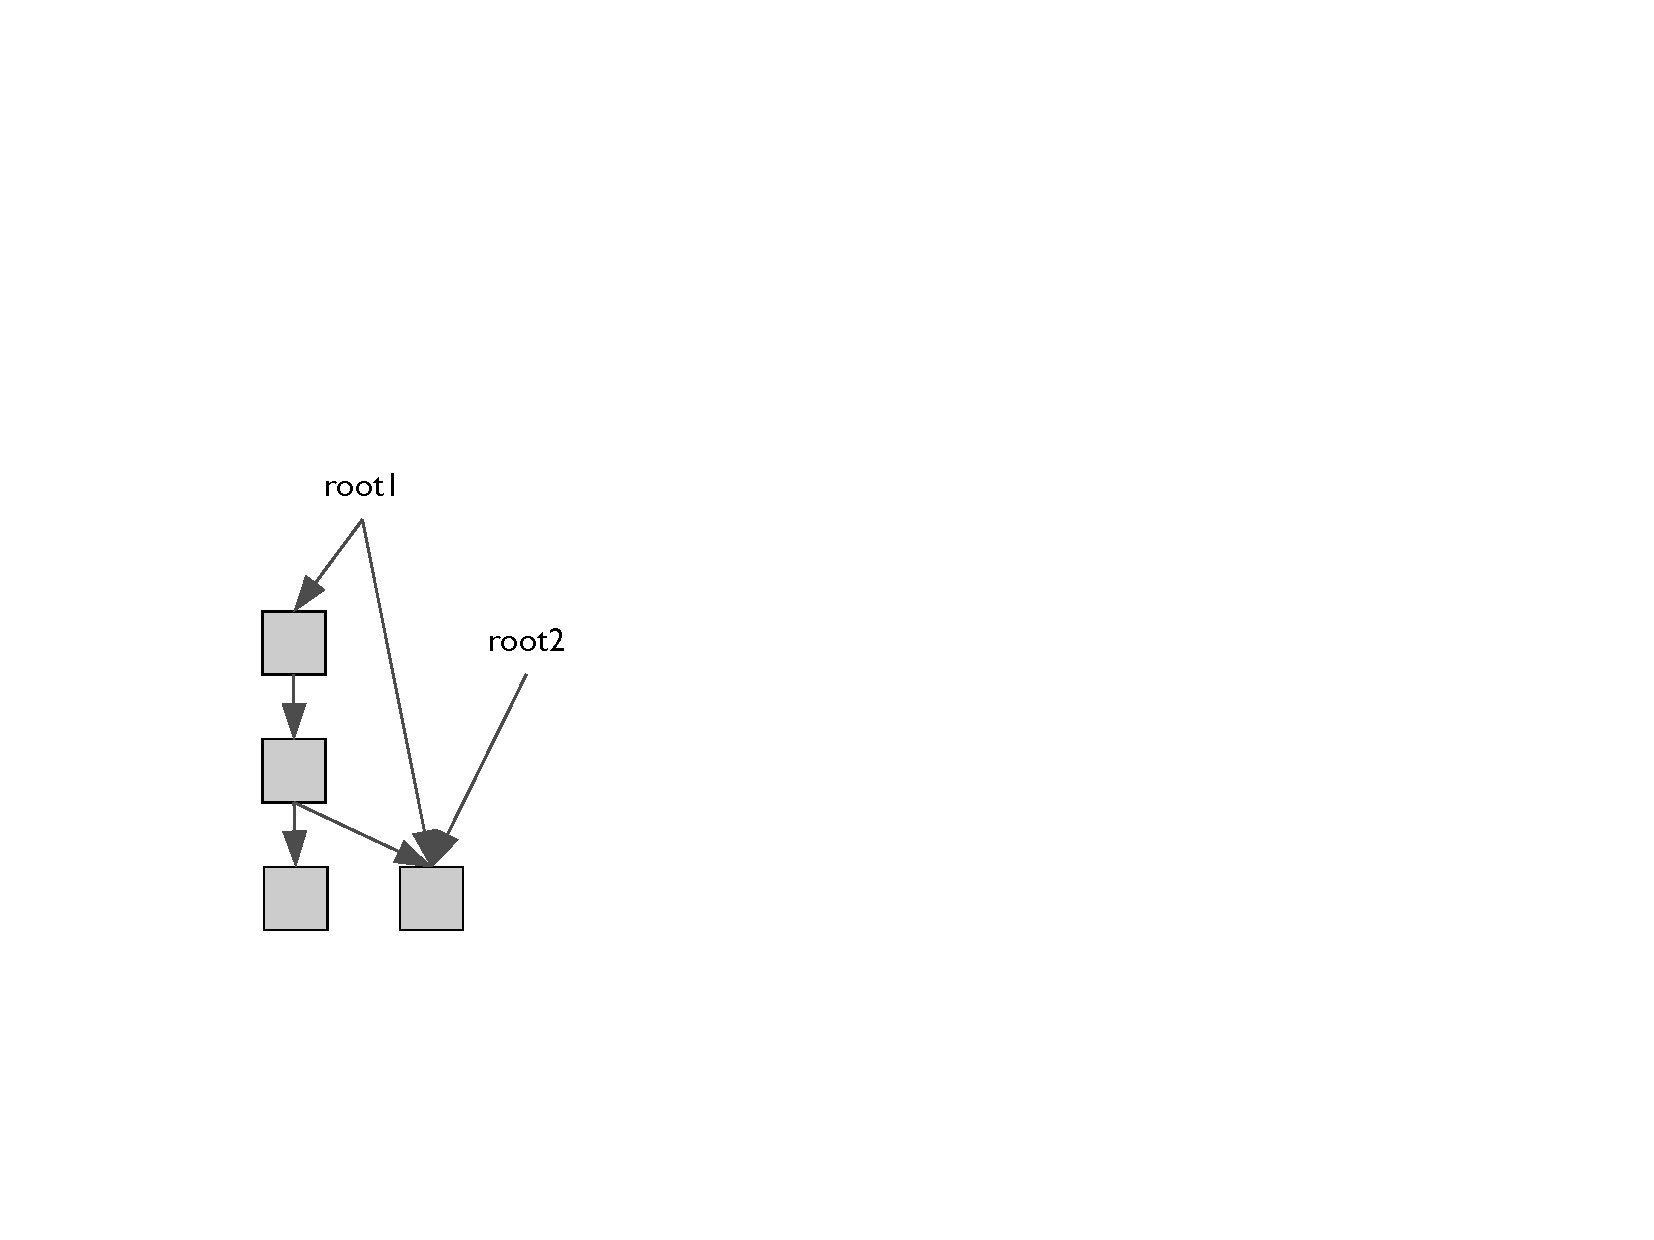
\includegraphics[width=0.3\textwidth]{part4/Figures/lifetime/reachability1}}
	\hspace{0.18\textwidth}
	\subfigure[Then, the dominating reference is
	clipped.]{\label{fig:reachability-b}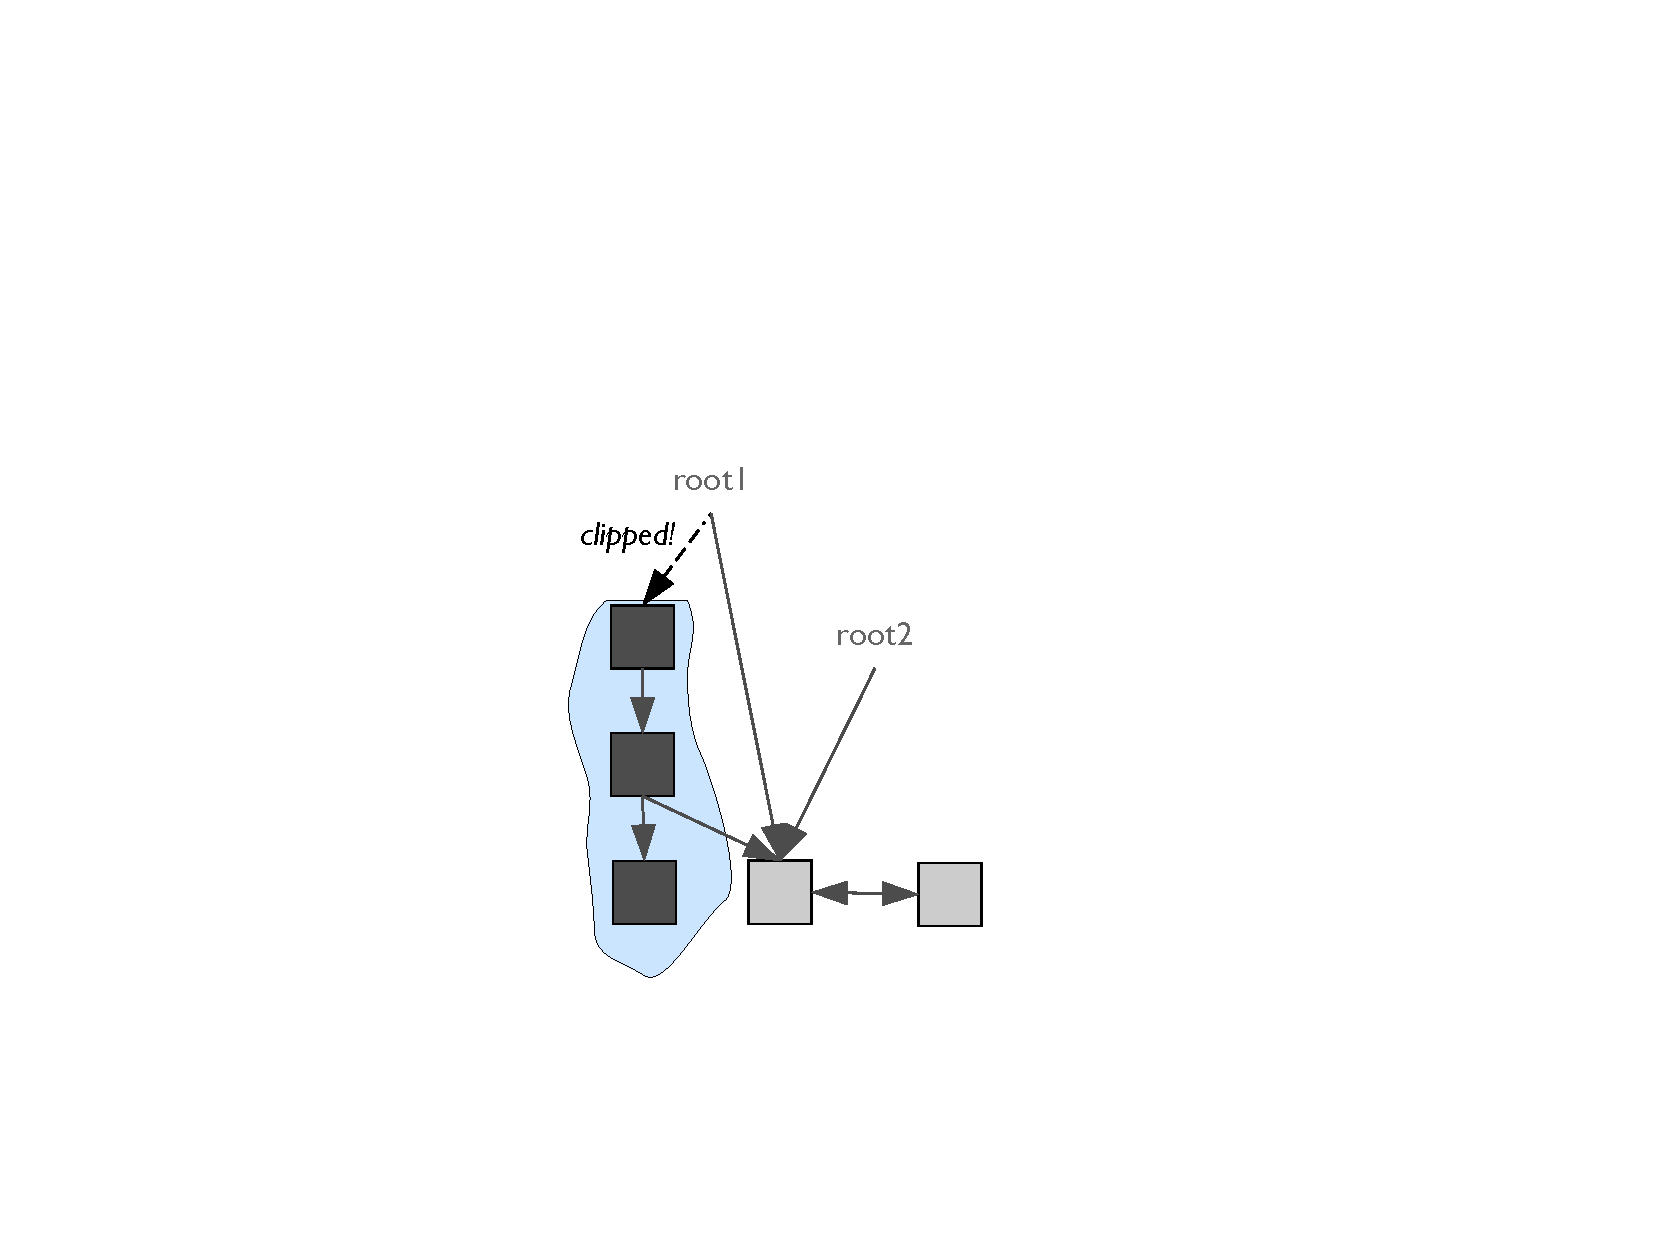
\includegraphics[width=0.445\textwidth]{part4/Figures/lifetime/reachability2}}
	\caption{The garbage collector uses the references between objects to
	determine what objects are collectable. The data structure on the left is
	filled entirely with live objects. The one on the right, after a link is
	clipped, now contains some collectable objects; all objects reachable only by
	traversing a \emph{dominating reference}, i.e. those \emph{dominated objects},
	will be collectable, as well.}
	\label{fig:reachability}
\end{figure}

This recursive aspect can also be expressed in terms of \emph{reachability}.
\index{Reachability} The live objects are those objects reachable, by following a
chain of references, from some root. \autoref{fig:reachability} illustrates a
simple data structure, and shows which part becomes collectable when a reference
is set to null, or ``clipped''. When the indicated reference is clipped, there is
no chain of references from a root to the shaded region of objects.

Reachability is the graph property that determines what objects are still live.
This is all the garbage collector cares about, finding the objects that need to
be kept around. It is also helpful for programmers to know which objects become
dead as the result of a pointer being clipped. The objects within the shaded
region of \autoref{fig:reachability-b} have the property that each is reachable
\emph{only} from the clipped reference. That clipped reference is the unique
owner of the shaded objects. The graph property that describes unique ownership
is called \emph{dominance}; \index{Dominance} the clipped reference is said to
dominate those objects that it uniquely owns.

\paragraph{The Collection Schedule and Safe Points}
The garbage collector does not reclaim memory immediately after an object's last
use. Instead, to amortize the costs involved in reclamation, the garbage
collector often lets reclaimable objects pile up for a while, and reclaims memory
in bulk. This bulk operation or reclaiming unused memory is usually implemented
as a number of threads. These worker threads, on some schedule, wake up and
traverse the heap for live objects. As objects are allocated, memory consumption
can be observed to increase, up until some maximum allowed amount. At this point,
the collector reclaims unused memory, and the process starts again. In this way,
memory consumption over time often assumes a sawtooth edge, such as those shown
in \autoref{fig:timeline-base-session-temps-with-cache}.
\index{Sawtooth Pattern}

\paragraph{GC Safe Points}
\index{Safe Points, use for Garbage Collection}

In most production \jres, garbage collection is, in normal execution, not run at
arbitrary points in the code. For example, in the above method \code{Foo.bar},
even though the object referred to by \code{localVariableReference1} becomes
unreachable before the end of the invocation, most \jres will not notice this
until a period of time after the assignment to \code{null} at line 6. This delay
comes about because the garbage collector typically only runs when threads reach
certain \emph{safe points} in the code. Safe points commonly include the
beginning or end of method invocations, the end of each loop iteration, and
points surrounding native method invocations. Therefore, the earliest time at
which the object referred to by \code{localVariableReference1} could be reclaimed
is after the first iteration of the loop; it could even possibly be the end of
the invocation, if the loop iterates zero times.

This is not to say that the garbage collector runs at every safe point, or that
it waits for all threads to reach a safe point before proceeding. Any thread that
tries, but fails, to allocate a new object will of course result in a garbage
collection at whatever line of code that allocation is found. At that point in
time, the other threads will continue executing up until their next safe point,
or their own failure to allocate memory, at which point garbage collection can
proceed.

\index{Safe Points, use for Garbage Collection}

In most production \jres, garbage collection is, in normal execution, not run at
arbitrary points in the code. For example, in the above method \code{Foo.bar},
even though the object referred to by \code{localVariableReference1} becomes
unreachable before the end of the invocation, most \jres will not notice this
until a period of time after the assignment to \code{null} at line 6. This delay
comes about because the garbage collector typically only runs when threads reach
certain \emph{safe points} in the code. Safe points commonly include the
beginning or end of method invocations, the end of each loop iteration, and
points surrounding native method invocations. Therefore, the earliest time at
which the object referred to by \code{localVariableReference1} could be reclaimed
is after the first iteration of the loop; it could even possibly be the end of
the invocation, if the loop iterates zero times.

This is not to say that the garbage collector runs at every safe point, or that
it waits for all threads to reach a safe point before proceeding. Any thread that
tries, but fails, to allocate a new object will of course result in a garbage
collection at whatever line of code that allocation is found. At that point in
time, the other threads will continue executing up until their next safe point,
or their own failure to allocate memory, at which point garbage collection can
proceed.


\paragraph{Configuration Settings}
You can guide the frequency of collection, which will change the slope of this
sawtooth curve to be either more or less jagged. In one common case, the garbage
collector will wait until all available memory is consumed before reclaiming
storage.  In Java, you can configure this ceiling by supplying a sizing to the
\code{-Xms} (initial ceiling) and
\code{-Xmx} (maximum ceiling) command line options. \index{-Xms command line setting}
\index{-Xmx command line setting} The \jre will begin with a ceiling at the
former level. If collections are occuring too frequently, the \jre may decide to
increase the \emph{current} ceiling to a higher level. As the need for memory
fluctuates, so the \jre will raise or lower the current ceiling level. The
current ceiling will always be some value lower than the maximum, \code{-Xmx},
setting. One such scenario, of increasing ceiling level, is illustrated in
\autoref{fig:timeline-base-session-temps-with-leak}.

\paragraph{The Nursery and Mature Heaps}
\index{Nursery}

\begin{figure}
\centering
	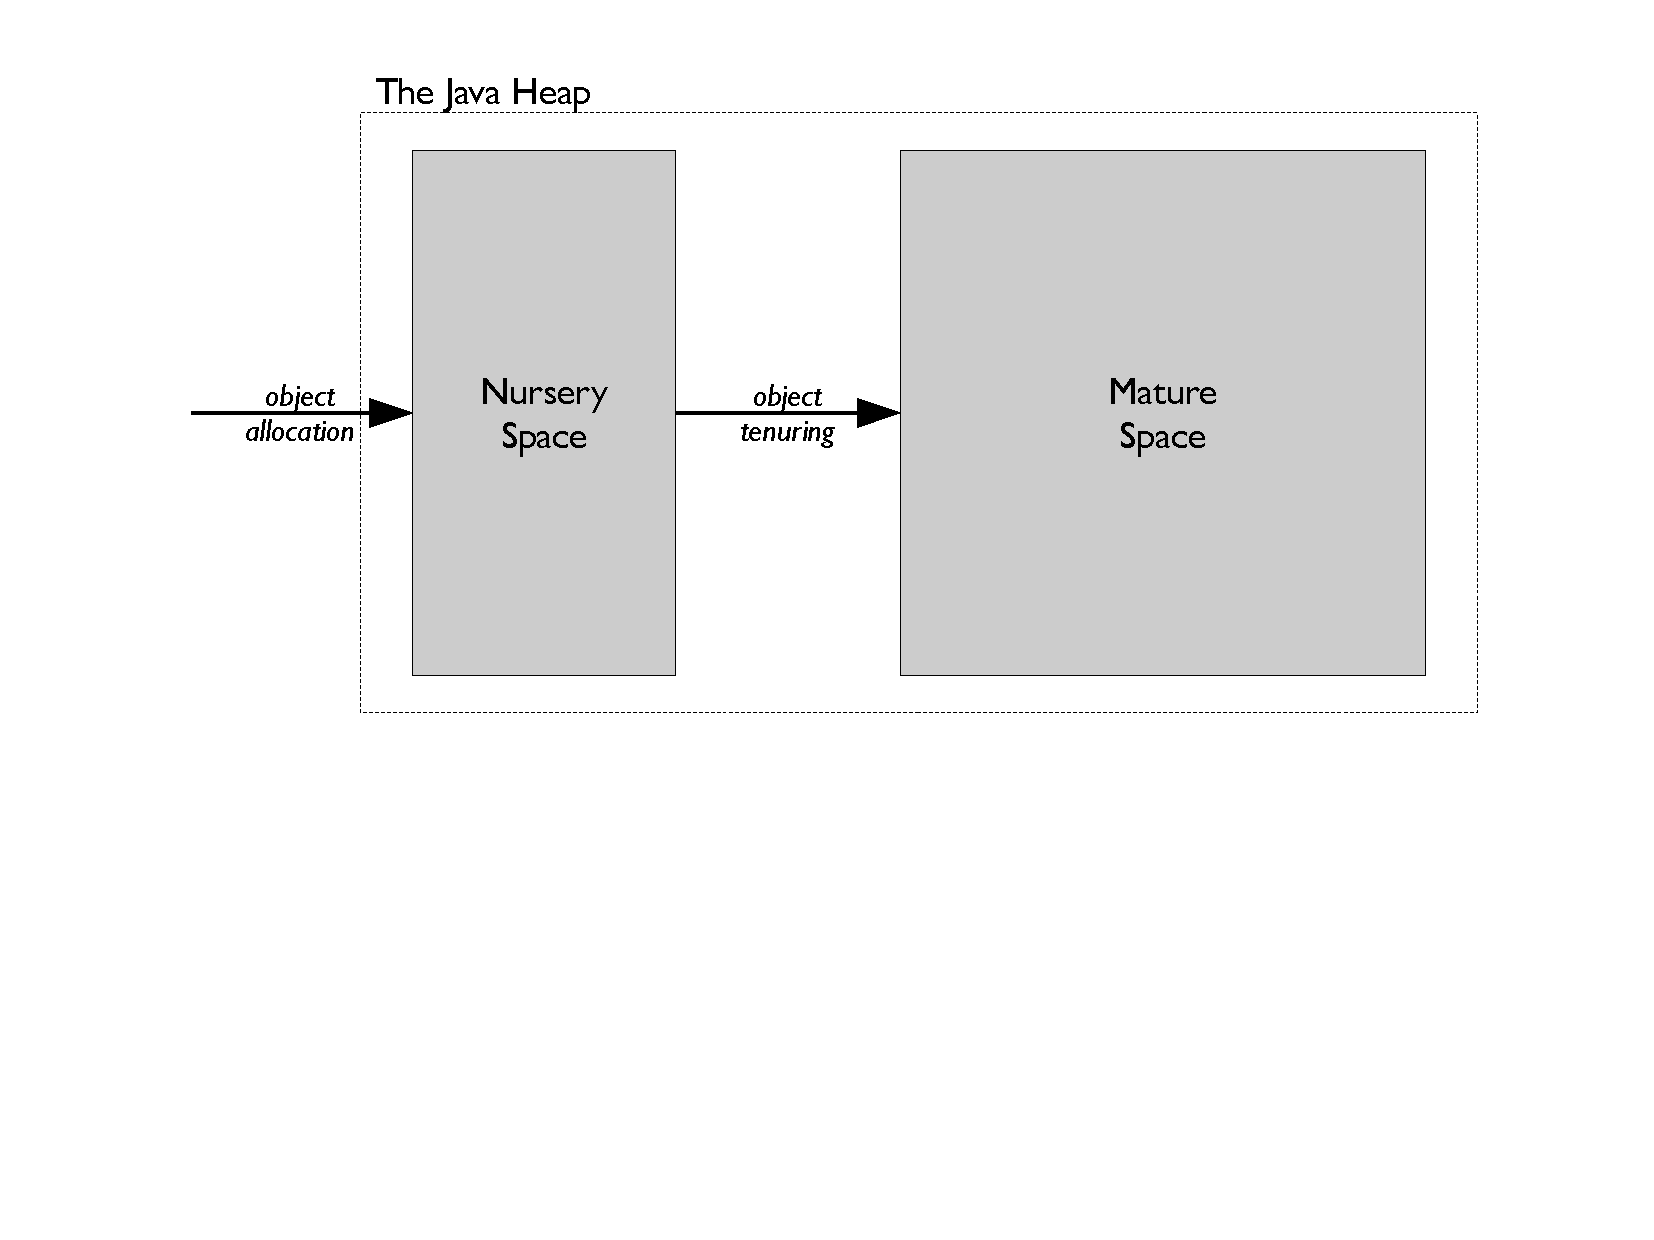
\includegraphics[width=0.6\textwidth]{part4/Figures/nursery}
	\caption{Oftentimes, the Java heap is split into two sub-heaps. The nursery
	space stores newly-allocated objects, and the mature space stores objects that
	have been tenured. The garbage collector tenures an object after it
	survives a sufficient number of nursery garbage collections.}
	\label{fig:nursery-and-mature}
\end{figure}

To optimize for applications that create a large number of temporary objects,
some garbage collection strategies attempt to separate the short-lived and
long-lived objects into two separate heaps. These two heaps are typically called
the \emph{nursery} and \emph{mature} spaces, as illustrated in
\autoref{fig:nursery-and-mature}. The usual behavior is for objects to be
allocated in the nursery and, if they survive a sufficient number of garbage
collection cycles, to be \emph{tenured} to the mature space. If a large majority
of the objects in the nursery are no longer live at the time the \jre runs a
garbage collection on the nursery heap, then a traversal of the nursery help will
only touch a small number of memory pages. In this way, ignoring the costs of
initialization, reclaiming objects that are short-lived can be very cheap. Some
collectors allow you to specify a separate maxmum size for each, and some let you
specify only the maximum nursery size and the total maximum heap consumption (via
\code{-Xmx}.)

\paragraph{The Permspace Heap}
\index{Constant Pools}
\index{Permspace}
In addition to separating new and old objects, some \jres create
a third heap in which to store data that is very unlikely to ever become
garbage. This includes the \jres metadata for your Java classes, along with the
executable code for your methods. In addition, any strings that you have
interned will be stored in this heap, along with any objects that the source
code compiler has decided to store in the \emph{constant pool} for a class;
these objects include any static strings, such as the one in this code snippet:

\begin{shortlisting}
System.out.println("aStaticString");
\end{shortlisting} 

The maximum size of Permspace, like the other heaps in Java, can often be
specified on the command line. In some cases, you may find that your application
requires a suspciously large maximum size for Permspace.
 
\begin{example}{Class Duplication and Excessive Permspace}
A Java Enterprise Edition (JEE) server application is deployed as 100 separate
applications, each in its own Web Application Archive (termed \code{war}) file.
Each \code{war} file contains duplicate class files for logic common to some, or even all applications.
The development team didn't think to worry about this, figuring that the
\jre would notice and remove the duplication. They were wrong, due to
requirements of the JEE specification, and suffered from excessive Permspace
consumption.

In JEE, each \code{war} file represents a distinct application, probably
separately developed. Having been coded separately, the JEE model assumes the
worst, that the applications will collide in their use of the static fields of
classes. Therefore, each \code{war} is loaded into a separate classloader, with
the result that the class duplication is not removed. The server application
required 500 megabytes for its Permspace heap, despite having under 100 megabytes
of distinct class data.
\end{example}


%% DO WE NEED THIS?
%\paragraph{Concurrent, Parallel, and Real-time Collection}
%\index{Concurrent GC}
%\index{Parallel GC}
%\index{Real-time GC}

\section{How to Free an Object in Java}
\label{sec:natural-lifetime}
\index{Natural Lifetime of Objects}

If you wish an object's storage to be reclaimed, you must take some care. To do
so in a language like C is simple, if bug prone. When you call \code{free} on any
pointer to a dynamically allocated memory region, memory is immediately available
for subsequent use.\footnote{It is possible to run a C program with a
special \code{malloc} library that introduces a simplified form of garbage
collection.} A C style of memory management comes with well known risks, and
commonly leads to memory errors. For example, memory might be deallocated more
than once, or variables that do not point to the start of an allocated region
might be passed to \code{free}. Still, using \code{free} is straightforward to
use, and immediate in effect.

In Java, you are immune from these problems, but there is no way to return memory
for immediately use in future allocations. Instead, you indicate, either
implicitly or explicitly, that objects are no longer needed. The explicit
mechanism is to set references to null. To do so implicitly, there are several
devices at your disposal. This section describes the details of both.

It is important to remember that in contrast to C, all means of indicating an
object is no longer needed have a certain degree of delay. There are delays of
two sorts. First, if you rely on the implicit mechanisms for indicating an object is no
longer needing, there is often a delay from its last use to this point. Second,
there is a delay from the point at which you indicate an object is no longer
needed until its storage is reclaimed.

\paragraph{The Lifecycle of an Object}
These two delays are but a part of the larger lifecycle that every Java object
goes through, from creation to reclamation. In a well-behaved application, an
object's lifetime spans its allocation, use, and the short period during which
the \jre takes control and reclaims the space. For some subset of an object's
actual lifetime, that is the time from creation to reclamation, your application
will make use of the data stored in its fields. \autoref{fig:typical-lifecycle}
illustrates the lifecycle of a typical object in a well behaved application.

\begin{figure}
	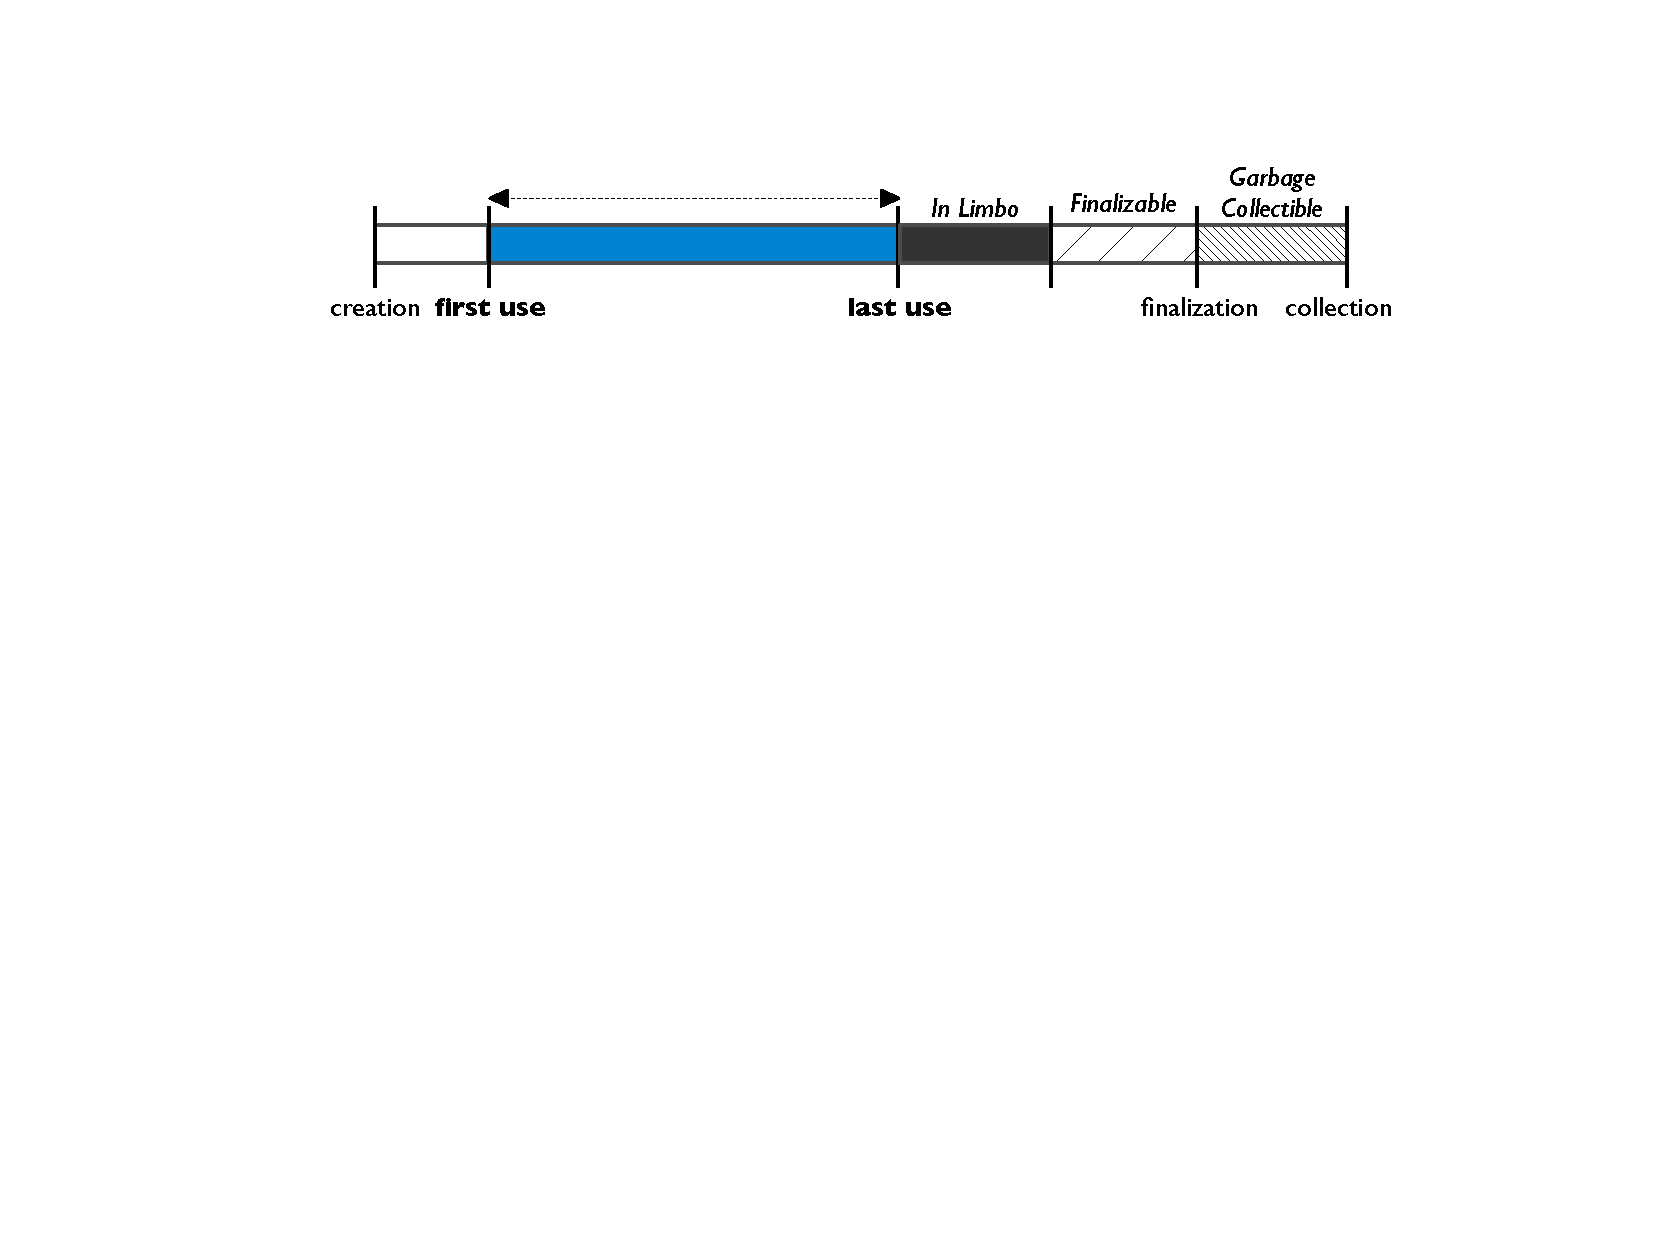
\includegraphics[width=0.9\textwidth]{part4/Figures/lifetime/object-lifecycle}
	\caption{Timeline of the life of a typical object.}
	\label{fig:typical-lifecycle}
\end{figure}


\begin{example}{Parsing a Date} Consider a loop that shows an easy way to parse
a list of dates. What objects are created, and what are their lifetimes?
\begin{shortlisting}
for (String string : inputList) {
	ParsePosition pos = new ParsePosition(0);
	SimpleDateFormat parser = new SimpleDateFormat();
	System.out.println(parser.parse(string, pos));
}
\end{shortlisting}
\end{example}

For each iteration of this loop, this code takes a date that is represented as a
string and produces a standard Java \class{Date} object. In doing so, a number of
objects are created. Two of these are easy to see, in the two \code{new} calls
that create the parse position and date parser objects. The programmer who wrote
this created two objects, but many more are created by the standard libraries to
finish the task. These include a calendar object, number of arrays, and the
\class{Date} itself. None of these objects are used beyond the iteration of the
loop in which they were created. Within one iteration, they are created, almost
immediately used, and then enter a state of drag.

\callout{drag}{Memory Drag}{
\index{Drag}
At some point, an object will never be used again, but the \jre doesn't yet know
that this is the case. The object hangs around, taking up space in the Java heap
until the point when some action is taken, either by the \jre or by the
application itself, to make the object a candidate for reclamation. The interval
of time between its last use and ultimate reclamation is refered to as
\emph{drag}.}

The \code{pos} object represents to the parser the position within the input
string to begin parsing. The implementation of the \code{parse} method uses it
early on in the process of parsing. Despite being unused for the remainder of the
parsing, the \jre does not know this until the current iteration of the loop has
finished. For this duration of time the object is in a kind of limbo, where it is
referenced but never be used again. This limbo time also includes the entirety of
the call to \code{System.out.println}, an operation entirely unrelated to the
creation or use of the parse position object. Once the current loop iteration
finishes, these two objects will become candidates for garbage collection.

\begin{figure}
	\centering
	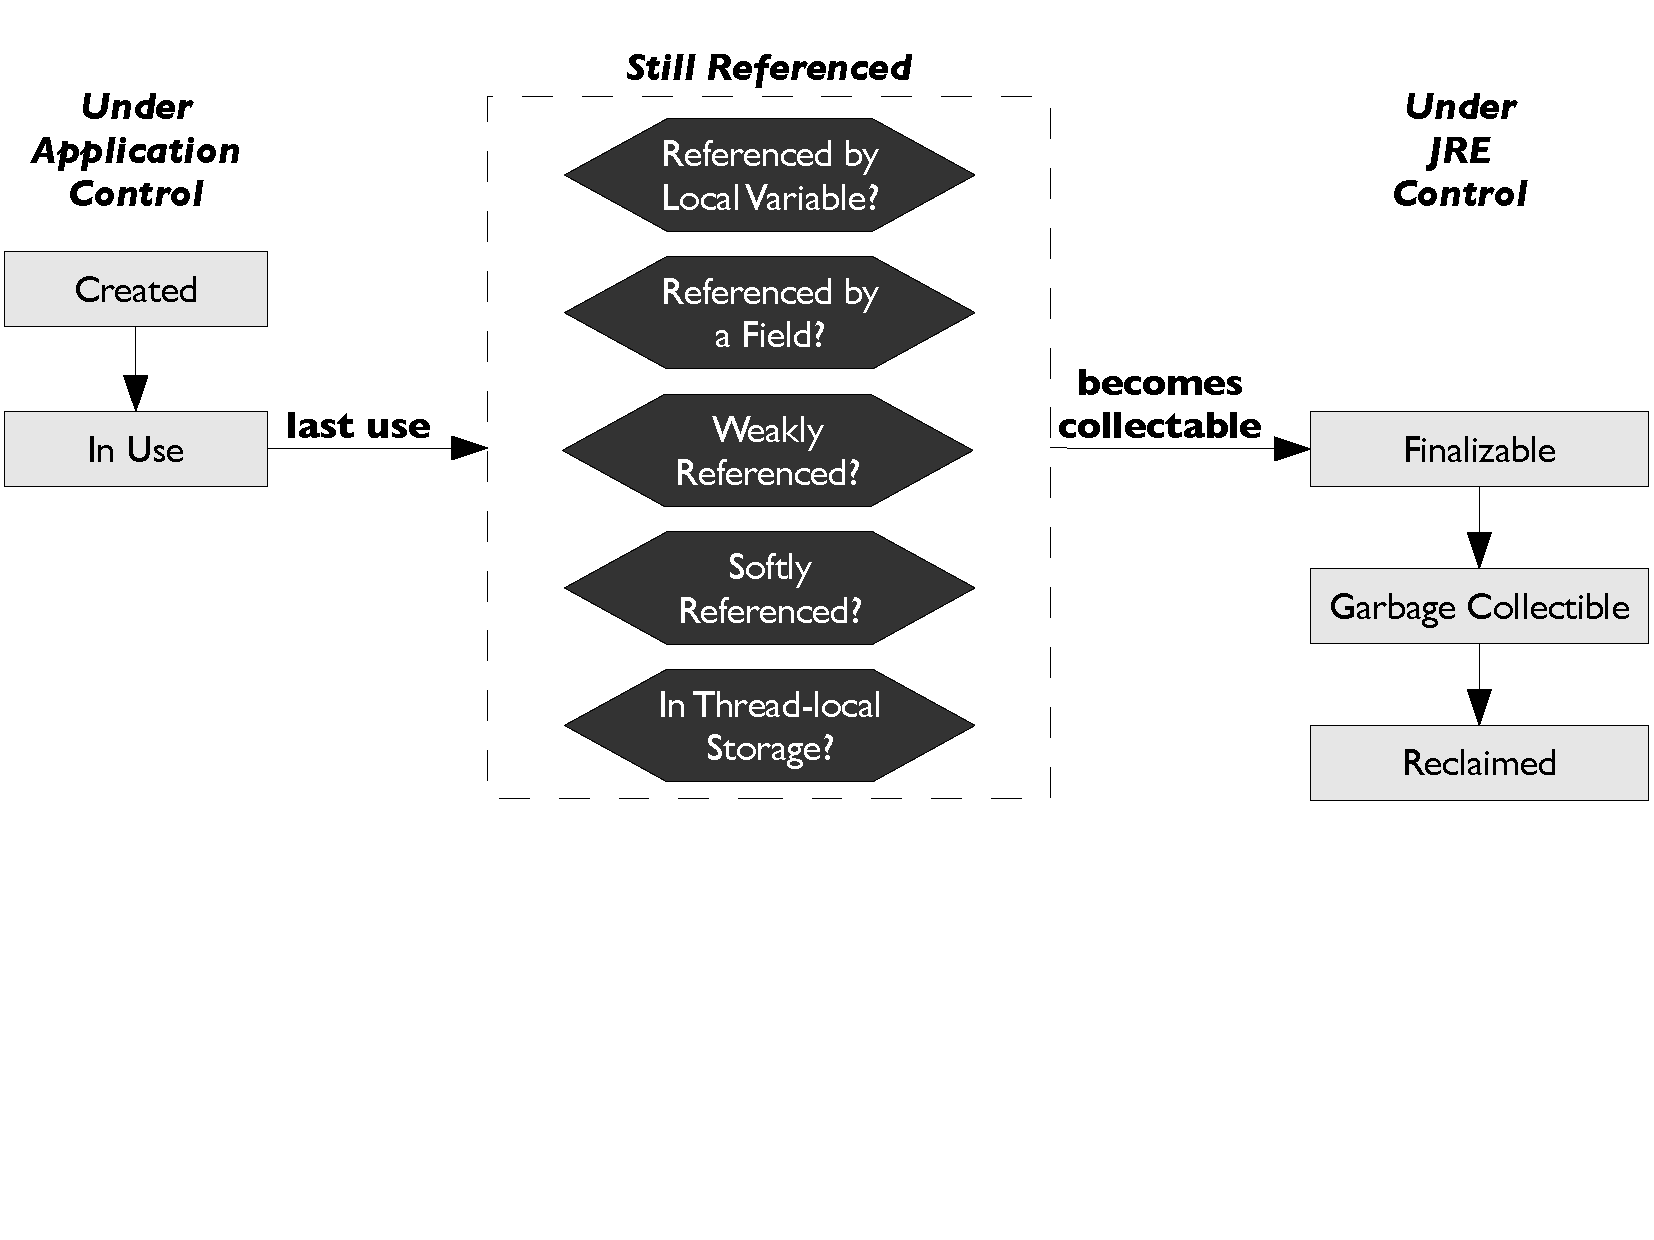
\includegraphics[width=\textwidth]{part4/Figures/lifetime/states}
	\caption{After its last use, an object enters a kind of limbo: the application
	is done with it, but it is not yet a candidate for garbage collection. When an
	object exits this limbo depends on the way it is referenced by your
	application.}
		\label{fig:limbo-exit}
\end{figure}

Depending on how the object is referenced by your application, it will
transition from in-use to garbage-collectable in a different manner. There are
eight ways an object may be referenced. It can be referenced by a:

\begin{enumerate}
  \item local variable of a method
  \item static field of a class
  \item instance field of a \class{java.util.ref.WeakReference} object
  \item instance field of a \class{java.util.ref.SoftReference} object
  \item instance field of a \class{java.util.ref.PhantomReference} object
  \item \tls
  \item instance field of any other object
  \item some combination of the above
\end{enumerate}

The first seven are cases of unique ownership of an object. There exists
only one path, via that particular reference, to reach the object. The eight case
is one of \emph{shared} ownership. After your program creates an object, it
references the object in one or more of these eight ways. The ownership of an
object may vary over time --- as your program runs, these references will come
and go. After some time, program execution may reach a point where the object is
no longer under application control. At this point, the \jre is now in charge of
its lifetime. For example, if the only reference to an object is from a field of
some other object, and your code reassigns that reference to \code{null}, this
becomes a point of transition, from application control to \jre control. Each of
the eight ways of referencing an object comes with its own guidelines as to when
this transition occurs. \autoref{fig:limbo-exit} and \autoref{tab:limbo-exit}
summarize how an object transitions to \jre control. The following code gives
examples of these eight patterns of ownership:
\lstset{numbers=left,numbersep=12pt,numberstyle=\tiny\textsf}
\begin{shortlisting}
class Foo {
   void bar(Object argument) {
      Object localVariableReference1 = new ...;
      threadLocal1.set(argument);
      threadLocal2.set(new ...);
      localVariableReference1 = null;
      for (...) {
         Object localVariableReference2 = new ...;
         ...
      }
   }

   static Object staticField = new ...;
   Object instanceField = new ...;
   Reference weak = new WeakReference(instanceField);
   Reference soft = new SoftReference(instanceField);
   Reference phantom = new PhantomReference(instanceField);
   ThreadLocal threadLocal1 = new ThreadLocal();
   ThreadLocal threadLocal2 = new ThreadLocal();
}
\end{shortlisting}
\lstset{numbers=none}
% Still, one can't always rely on automatic mechanisms to guide an object out of
% limbo in a timely fashion.

\begin{table}
\centering
	\begin{tabular}{ll} \toprule uniquely owned by  & 
	when object becomes candidate for reclamation \\ \cmidrule(r){1-1}
	\cmidrule(l){2-2}
			%
			nothing & immediately
        	\\
        	%
        	local variable & after scope exits, e.g. method returns
        	\\ \addlinespace
        	%
        	instance field of an object & 
        	when that object becomes reclamation candidate
        	\\
        	%
        	static field of a class &
        	when that class is unloaded
        	%
        	\\ \addlinespace
        	field of \class{WeakReference} & immediately
        	%
        	\\
	       	\ldots with \class{ReferenceQueue} &
        	immediately placed on queue, then after queue is polled
        	%
        	\\ \addlinespace
        	field of \class{SoftReference} & approximately
        	LRU%$^{**}$
        	%
        	\\
	       	\ldots with \class{ReferenceQueue} &
        	after LRU, placed on queue, then after queue is polled
        	%
        	\\ \addlinespace
        	entry in \tls & when that thread dies
        	%
        	\\ 
        \bottomrule
    \end{tabular}
	\caption{When an object becomes a candidate for reclamation. The dominating 
	reference can be explicitly overwritten, e.g. by your code expliclty assigning the
	reference to \code{null}. Otherwise, an object only automatically becomes a
	candidate under the restricted circumstances shown here.
%	The point when an object exits limbo depends on 
	%decisions under programmer control: it depends on how the object is
	%referenced.
	%older {\jre}s	use very poor heuristics for handling soft references; see the
	% body for more detail.
	%, it will be reclaimed
	%under certain rules, or may be part of a memory leak
	}
	\label{tab:limbo-exit}
\end{table}

\paragraph{The Lifetime of Local Variables}
\label{sec:lifetime-of-locals}
Variables that are declared within a method body often have a lifetime that is
bound to, at most, the duration of an invocation of that method.
% If an object is uniquely owned by a local variable of a method, the \jre will
% begin to consider reclaming its storage no sooner than when the local
% variable's scope exits.
Common examples of this are local variables, loop variables, and variables
declared within some inner scope such as within the body of a loop or \code{if}
statement. For these variables, when a loop continues to the next iteration as in
the case of \code{localVariableReference2}, when the body of a clause of an
if/then/else statement finishes, or when the method invocation returns as in the
case of \code{localVariableReference1}, there is a good chance that the object
referenced by that variable will be reclaimable.

There are situations where an object may \emph{escape} the local scope in which
it was declared.\index{Escaping Objects} In these cases, the object has
\emph{shared ownership}\index{Shared Ownership} until this local scope exits.
See below for further discussion of shared ownership. This is an example of an
object escaping a local variable scope, so that it is, for the duration of that
local scope, also owned by a static field of a class object:
\begin{shortlisting}
class Foo {
   static Object static_obj;
   
   void foo() {
      Object obj = new Object();
      static_obj = obj;
      ... // uses of obj
   } // obj scope exits, but static_obj ownership persists
}
\end{shortlisting}
The next section discusses the lifetime of static fields.

The minimum that the Java language specification requires is that non-escaping
objects that are declared within some scope inside of a method will be
reclaimable by the time that scope exits. Many modern \jres try to optimize by
inferring, when they can, the line of code at which an object will certainly
never be used again. For this reason, some (but not all!) sources of memory
drag\index{Drag} that would have been a problem with older \jres, are no longer
an issue. For example, you can run this test program and, by inspecting the
output, determine whether your \jre is performing this kind of optimization:
\begin{shortlisting}
/* Test for whether the optimizer detects that obj is reclaimable before the end of this method */
static public void main(String[] args) {
   Object obj = new Object() {
      protected void finalize() {
         System.out.println("Finalized");
      }
   };
   System.out.println("StartOfLoop");
   for (int i = 0; i < 1000000; i++) {
       new HashSet().add(i);
   }
   System.out.println("EndOfLoop");
}
\end{shortlisting}
If you see the \code{Finalized} message before the end of loop message, this is a
sure sign that the \jre is being clever. Be careful to remember that seeing the
finalized message is definitive evidence, but not seeing that message might only
mean that your loop doesn't iterate enough times to cause a garbage collection to
occur. You may need to experiment with the number of loop iterations, before
coming to a conclusion.

\paragraph{The Lifetime of Statics, and Class Unloading}
\index{Class Unloading}
\index{Static fields}

The \jre allocates memory for every class, to store its static fields, such as
the one on line 13 in the above example. This memory, to store all static fields
plus some bookkeeping information, is often referred to as the \emph{class
object} for the class.\index{Class Objects} It is possible for the same class to
be loaded into multiple class loaders; in this way, using more than one class
loader lets you avoid the problem of colliding use of static fields in separately
developed parts of the code. A static field therefore only exits scope when the
class object is reclaimed, which occurs when the respective class is unloaded, by
the \jre, from its class loader. 

If a class is never unloaded, which is likely to the be case for your
application, then that class object will remain permanently resident. The
\emph{default} class loader, which is the one that will be used unless you
specify otherwise, never unloads application classes. 

If you need classes to be unloaded, then you must manually specify a class loader
to use. Unloading a class is then accomplished by ensuring that all references to
both the class object and your custom class loader, are set to \code{null}. This
will render the class unloadable, and will also render objects referenced by
static fields all classes loaded into that class loader as garbage collectable.
There exist module management systems, such as OSGi~\cite{OSGi_2007}, that
facilitate this task.

Due to these complexities, your design should generally anticipate that the
memory for these static fields is permanently resident. This means that any
static fields referencing an instance, rather than containing primitive data,
will render that instance also permanently resident. Unless, that is, you take
action to explicitly clip the static field reference, by assigning the field to
null. Otherwise, that instance will be forever reachable along a path from some
garbage collection root through the static field reference. In this way, storing
a reference in a \code{static} field of an class is one way to implement a
permanently resident lifetime policy.

\paragraph{The Lifetime of Instance Field References}

As long as an object \code{B} is dominated by an instance field of another object
\code{A}, then these two objects will live and die together. The only device at
your disposal to make \code{B} garbage collectable before \code{A} is to break
all paths of references from \code{A} to \code{B}. In simple cases, where
\code{B} is directly referenced by a field of \code{A}, then reassigning that
reference to \code{null} will do the trick. After doing so, the \code{B} object
will now be a candiate for garbage collection. 



%Every object created by your application lives for an interval of time from its
%creation to the point that the Java runtime gets around to collecting it. An object's {\em natural} lifetime is defined by the
%interval of time between its first and last necessary use. %cite drag paper
%here?








\begin{comment}
\begin{figure}
	\centering
%	\subfigure[The lifecycle of a typical object and its data.]{
	%\label{fig:typical-lifecycle1}
			%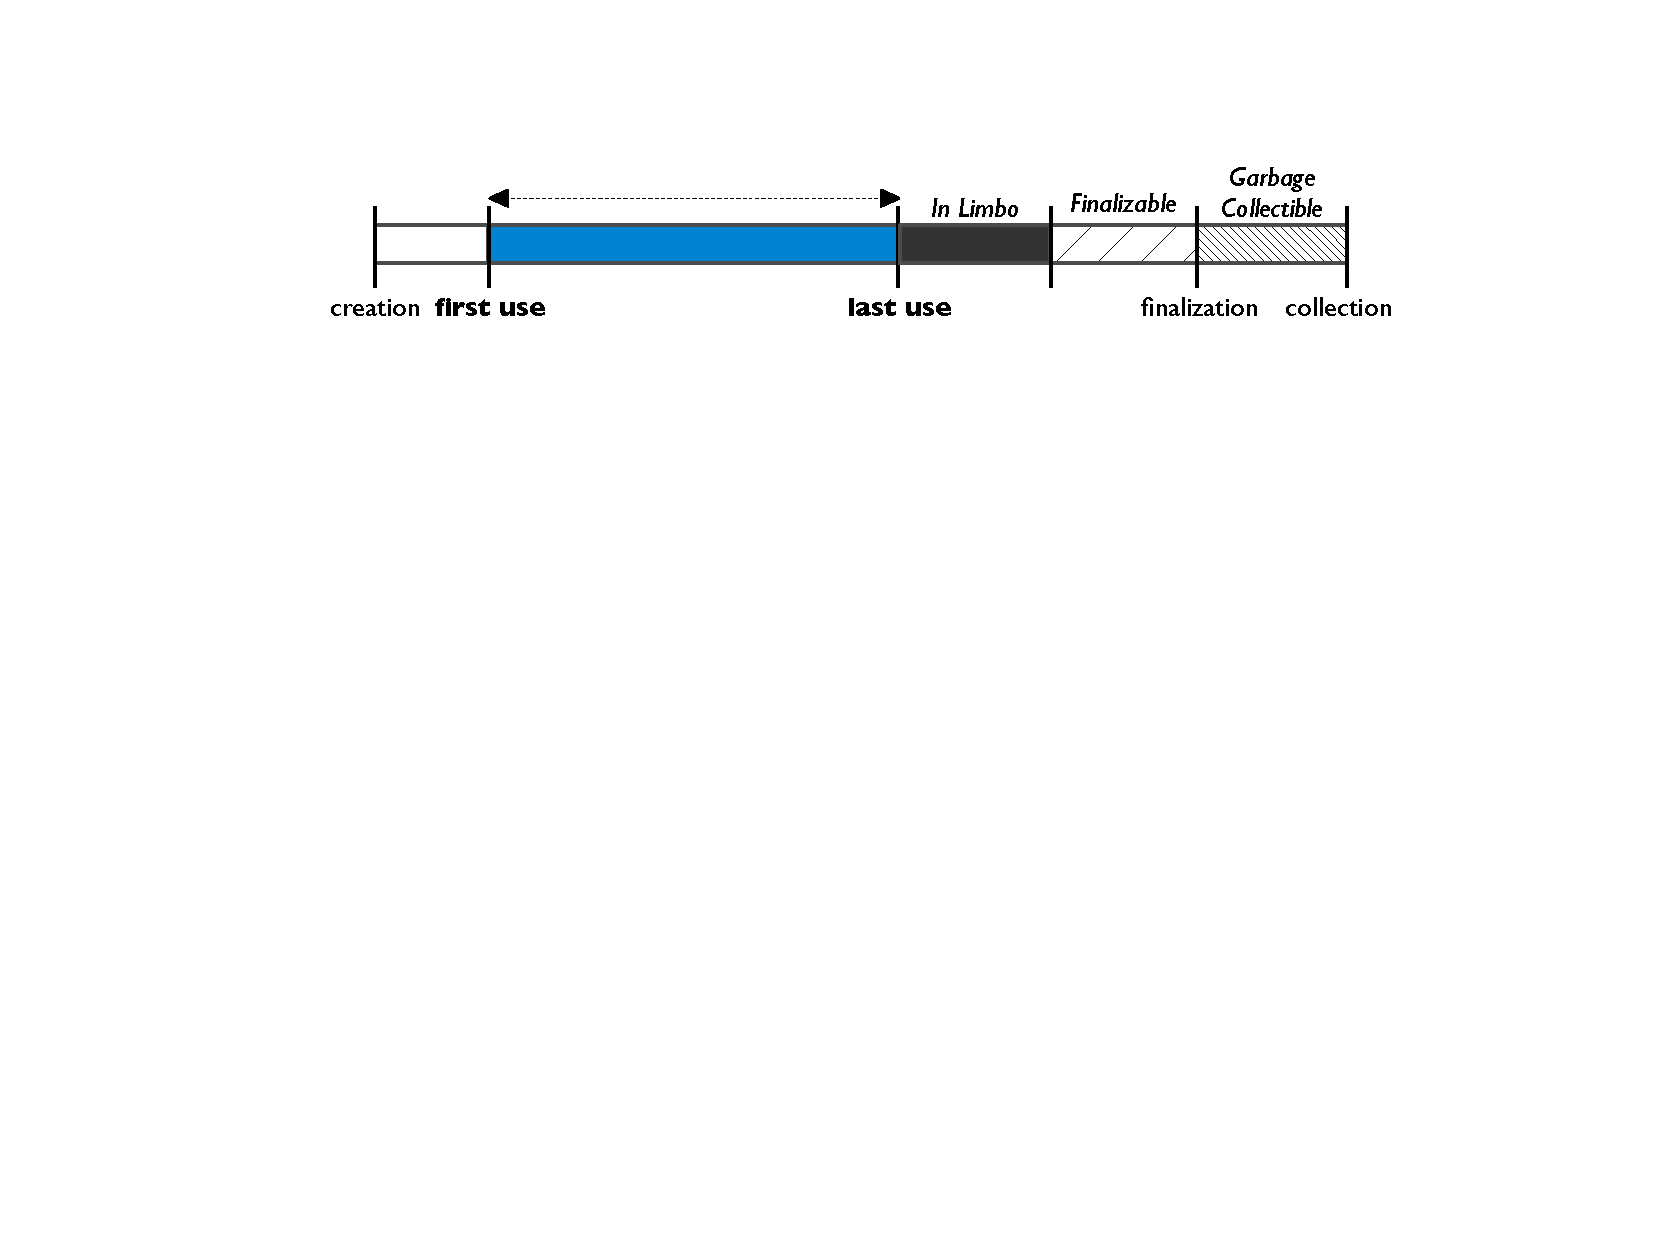
\includegraphics[width=0.95\textwidth]{part4/Figures/lifetime/object-lifecycle}
	%}
	\subfigure[A situation where there are long periods between uses of an
	object's data.]{
	\label{fig:typical-lifecycle2a}
		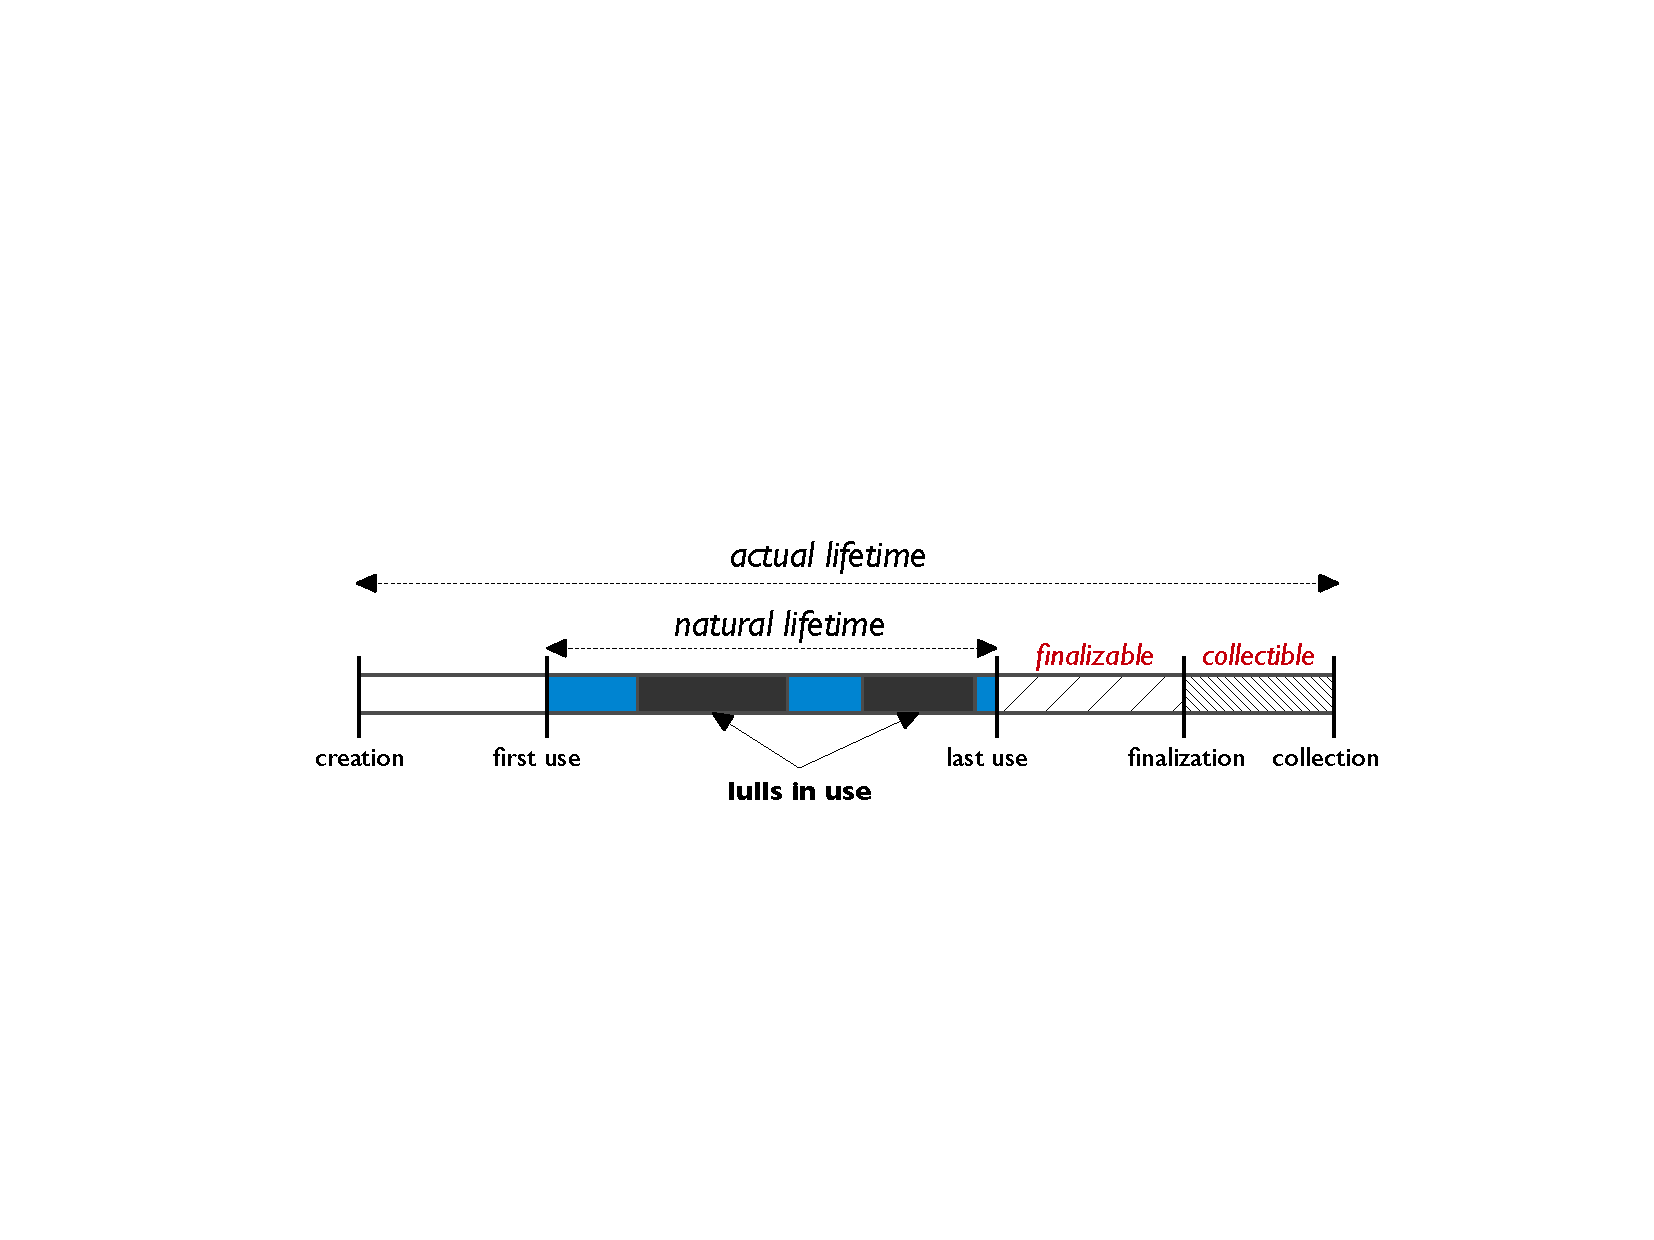
\includegraphics[width=0.95\textwidth]{part4/Figures/lifetime/object-lifecycle-lulls}
	}
	\subfigure[The lifecycle of the data  that is loaded from
	disk three times, and the objects that store it.]{
	\label{fig:typical-lifecycle2b}
		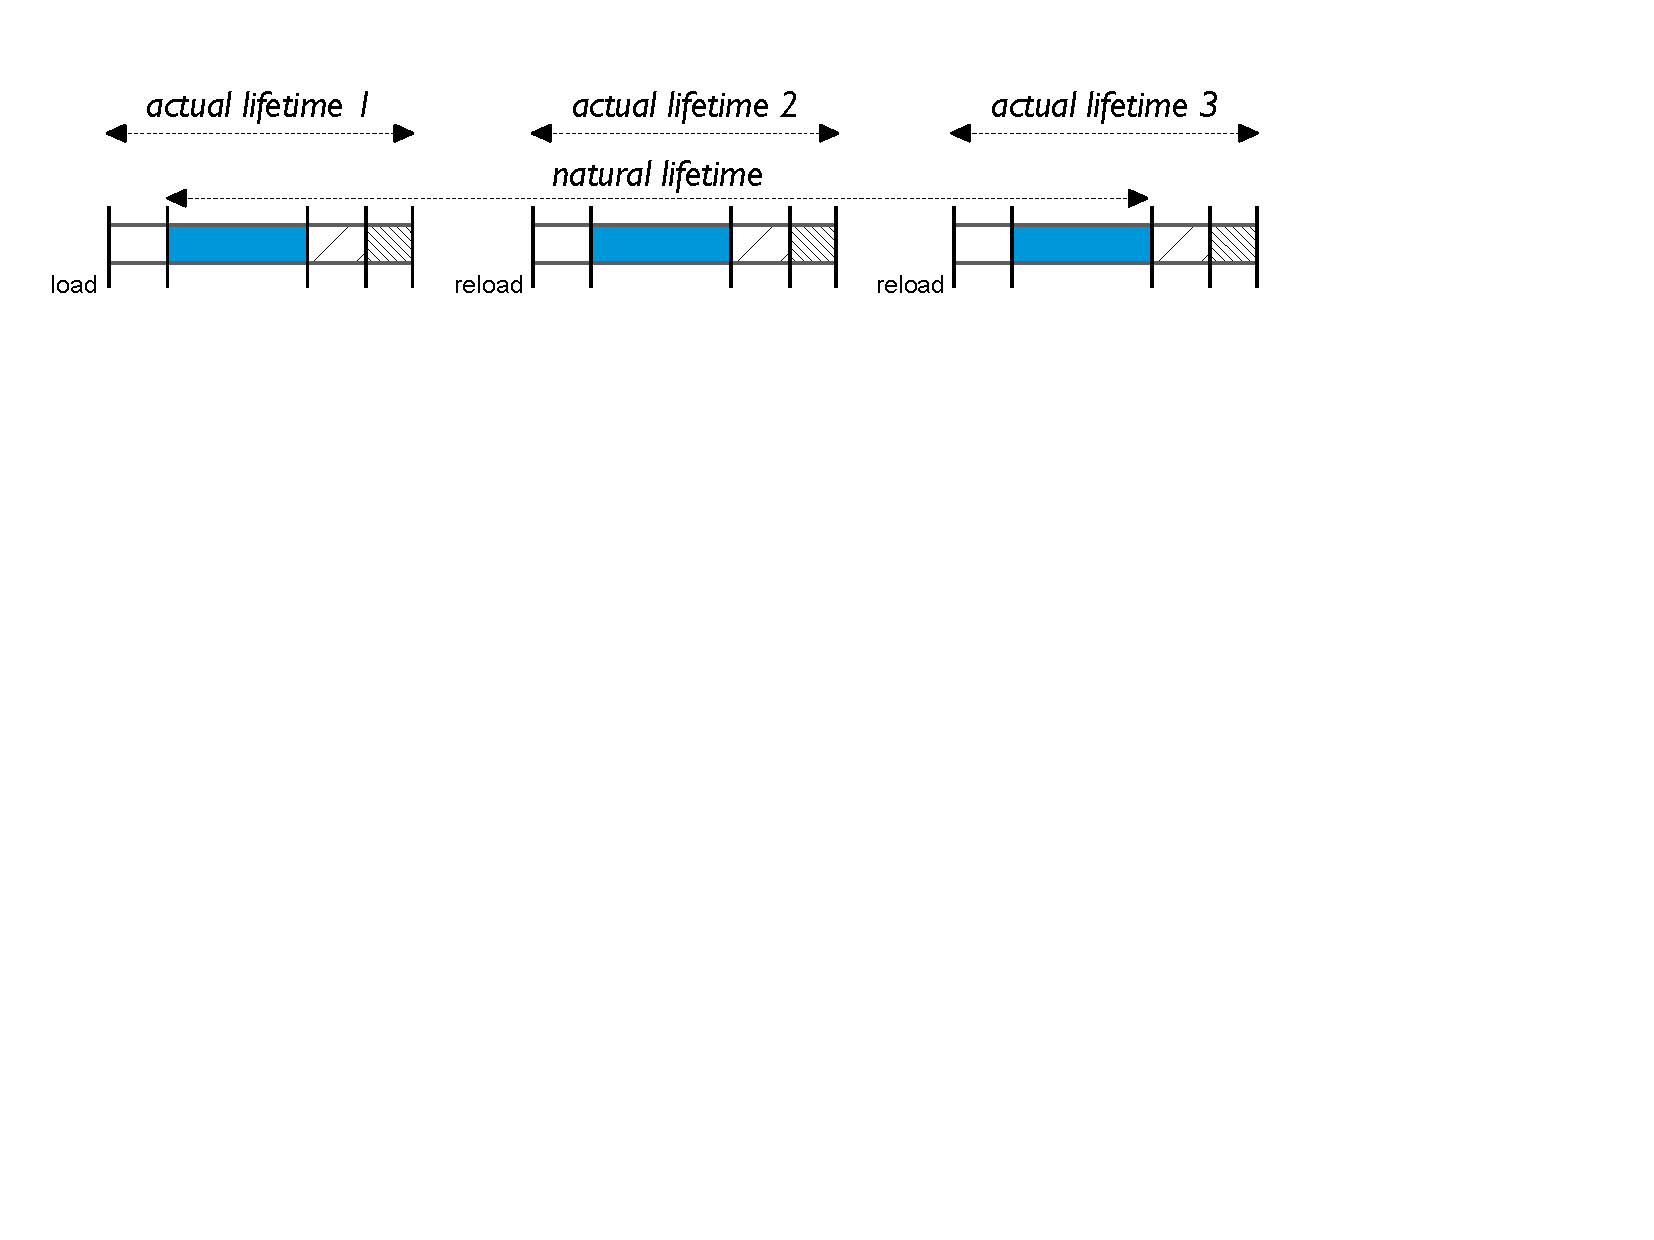
\includegraphics[width=0.9\textwidth]{part4/Figures/lifetime/object-lifecycle2}
	}
	\caption{Examples of Natural and Actual lifetimes.}
	\label{fig:typical-lifecycle2}
\end{figure}
\end{comment}


\paragraph{Shared Ownership}
\label{sec:shared-ownership}
\index{Shared Ownership}

When you invoke a library method, there is no way in Java to know what the called
method does with your object. It could very well squirrel away a reference to any
object reachable from arguments you pass to the invocation. Despite your best
efforts at keeping track of which references exist to an object, it can easily
become an uncontrolled mess once you pass these objects to third-party libraries.
In the above example, if you call the \code{parse} method of a
\class{SimpleDateFormat} object, the method contract says nothing about how it
treats the given string or \class{ParsePosition} passed as parameters. 
Consider the case where you need the string to become garbage collectable soon
after having parsed it, but the formatter maintains a reference in order to avoid
reparsing the same string in back to back calls. This calls
to mind the worst of the days of explicitly managing memory in a language like C.

In the case where there is more than one reference to the object, the story gets
more complicated. In contrast to C, where a \code{free} of \emph{any} pointer
suffices for deallocation, in Java \emph{all} references to an object must be
assigned to \code{null}. This is tricky in many cases, because it may not be easy
to know where all those references emanate from.
\autoref{fig:reachability-sharing} illustrates a situation where three references
must be clipped before an object, the darkly shaded one, becomes a candidate for
garbage collection. There are two other important things to note in this example.
First, just as in \autoref{fig:reachability-b}, after clipping the three
indicated references, an entire data structure, not just that darkly shaded
object, becomes a candidate for reclamation. This structure consists of the two
objects contained within the lightly shaded region. The second important thing to
note is that you needn't clip the backwards edge, or any edge contained entirely
within the data structure you no longer need.

\begin{figure}
\centering
\subfigure[Diamond sharing.]{
	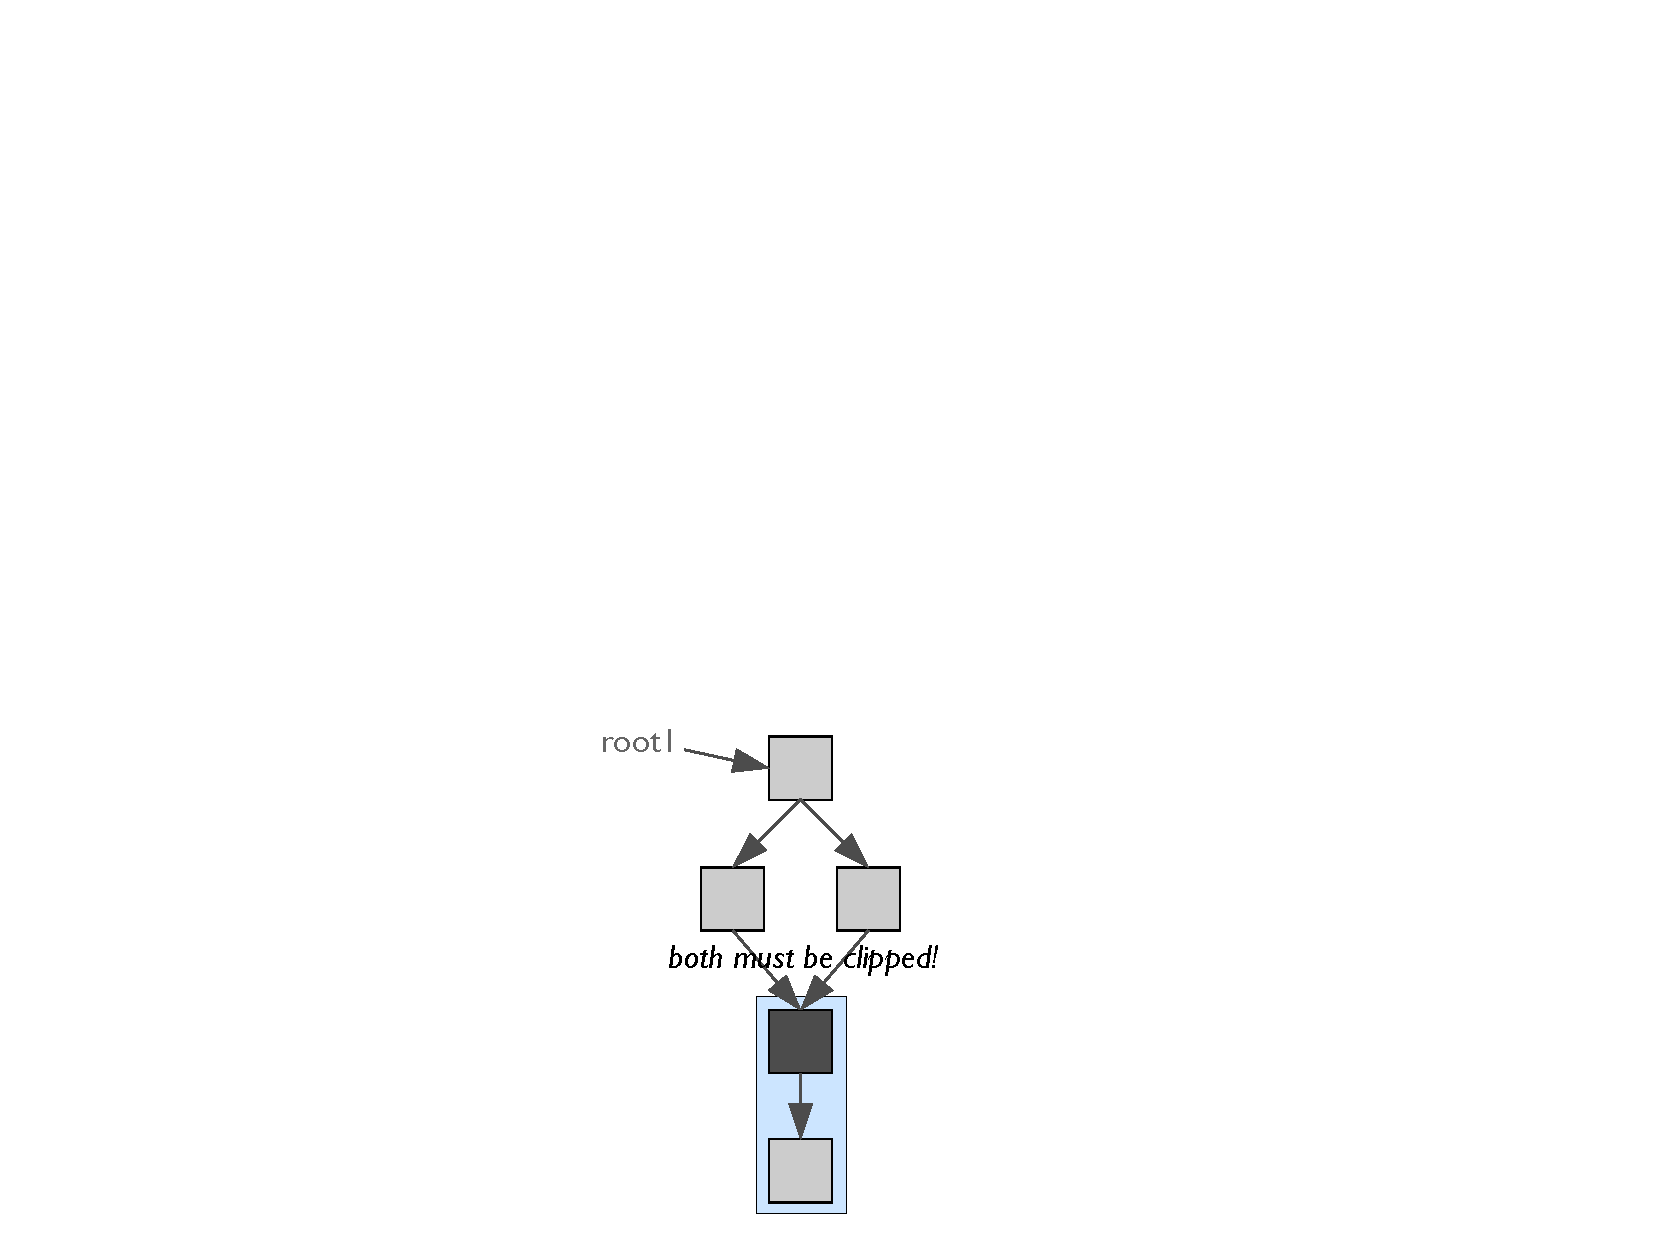
\includegraphics[height=0.25\textheight]{part4/Figures/lifetime/reachability4}
	}
\qquad
\subfigure[Root sharing.]{
	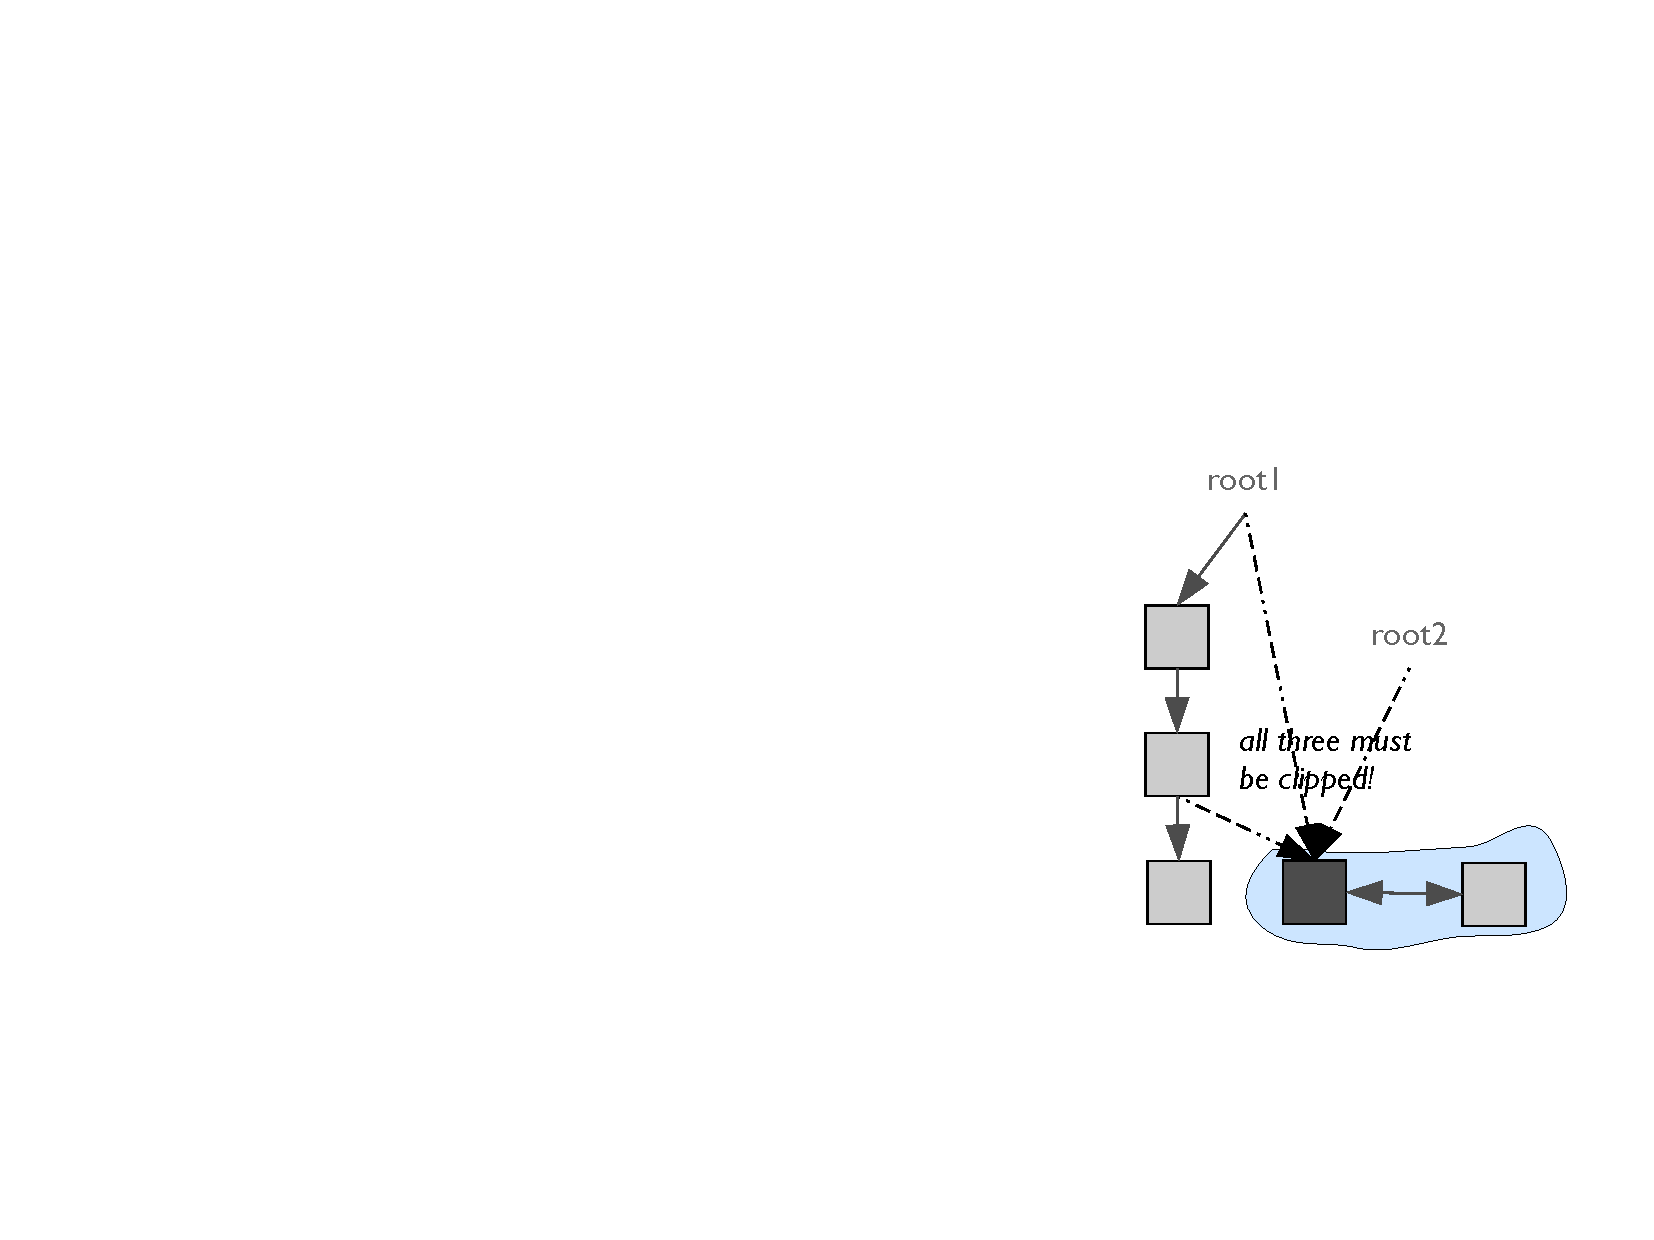
\includegraphics[height=0.22\textheight]{part4/Figures/lifetime/reachability3}
	}
	\caption{When an object is shared, such as the shaded ones shown
	here, care must be taken to clip all edges from emanating from outside of the
	region you wish to reclaim.}
	\label{fig:reachability-sharing}
\end{figure}

\section{Advanced Java Lifetime Management Features}
 
There are several important lifetime management policies that cannot be expressed
using normal mechanisms of local variables and static and instance field
references. For example, to implement the correlated lifetime policy described in
\autoref{sec:correlated-lifetime} using only the mechanisms presented so far is
difficult. In \autoref{fig:reachability-b}, there are three objects contained
within the shaded region; these three objects will all be garbage collectible if
the indicated dominating reference is set to \code{null}. In this way, the
lifetime of the lower two can be correlated with the lifetime of the object
directly pointed to by the dominating reference. This can work, in certain
limited circumstances, but it requires that you encode the correlation in the
class definition itself. To correlate an instance of the \class{B} class with an
instance of the \class{A} class, you must add a field to \class{A}:
\begin{shortlisting}
class A {
   B b;
}
\end{shortlisting}
In addition to requiring the pollution of class definitions, it also can result
in wasted memory. If only some \class{A} instances have a correlated \class{B},
then you will be wasting a pointer slot for every instance of \class{A}. It turns
out that this is how the Java standard \class{HashMap} was implemented, in its
mechanism for maintainin a correlation between the various views (the key set,
value set, and entry set), and the map itself:
\begin{shortlisting}
class HashMap {
   Set keySet, valueSet, entrySet;
}
\end{shortlisting}
This choice had a big implication on the memory bloat factor of small maps. As
we have learned in previous chapters, every instance of a standard Java hash map
must pay the expense for potential use of features. These features aren't
always employed, and certain rarely together, for a single map instance.

The Java language provides mechanisms that allow you more flexibility in
implementing lifetime management policies. These advanced features are exposed
via the \class{java.lang.ref.Reference} family of classes and \tls. Programmers
very often confuse these mechanisms, and there is quite a bit of disinformation
on the Internet; there is especially confusion over the use of soft and weak
references. Therefore, it is important for you to take some care in understanding
the low-level features.

To contrast the normal referencing mechanisms with these advanced features, the
normal ways of referencing objects are typically referred to as \emph{strong}
references. This term came about to contrast with the terms used for the more
advanced features: weak, soft, and phantom references.

\paragraph{Weak References (referencing an object without inhibiting its
reclaimability)}
\index{Weak References}

The constructor for a \class{WeakReference} takes an object as a parameter. The
resulting instance of \class{WeakReference} is said to \emph{weakly reference}
that other object. A weakly referenced object will be garbage collectable, or
not, independently of being referenced from the \class{WeakReference} object; the
weak reference provides a non-owning handle to another object. This is a
sometimes helpful combination, to be able to refer to the object, without
inhibiting it being reclaimed as it normally would. To tunnel through the level
of indirection introduced by the weak reference, you call its \code{get} method.
If this method returns \code{null}, then you know that the referenced object has
been reclaimed. \autoref{chapter:correlted-lifetimes} discusses how to leverage
this functionality for an alternative implementation of the correlated lifetime
pattern.

There are three issues that you must handle with care. First, even though the
weak reference itself does not prolong the lifetime of the referenced object,
once you call \code{get}, you now have a regular reference to that object. If
this reference is stored in a local variable, or in a field of another object, or
in a collection, then you have now altered its lifetime. Once normally
referenced, the underlying object now obeys the lifetime rules discussed earlier.
Second, you must be careful to avoid race conditions, such as:
\begin{shortlisting}
class A {
   WeakReference<B> b;
   
   B getB() {
      if (b.get() != null) {
         return b.get();
      } else {
         // perform any necessary cleanup
         // notify caller of b's reclamation
      }
   }
}
\end{shortlisting}
In that code, between the first call to \code{b.get()} and the second, the
underlying object may have been reclaimed. You must modify that code to call
\code{b.get()} only once, and stash the result in a local variable until
\code{getB} returns. Third, if you need to be informed that the underlying object
has been reclaimed, you must use the \emph{reference queue} mechanism, which will
be discussed shortly.

\paragraph{Soft References}
\index{Soft References}

The constructor for a \class{SoftReference} also takes an object as a parameter.
The object lives as it normally would until the point in time when there are no
other strong references to the object. When an object is only softly or weakly
referenced, then it enters a special transitionary lifetime state. The \jre will
keep this object around, for as long as there is enough free Java heap. Once heap
grows tight, the \jre will begin treating the soft references as if they were
weak references --- the soft references that the \jre choses to discard will no
longer inhibit the reclaimability of the softly referenced objects. This
discarding of soft references is sometimes referred to as ``clearing'' soft
references.

The Java language specification makes no specific requirements as to how \jre
implementations should chose which soft references to discard. The only
requirement imposed by the language specification is that the \jre must have
cleared \emph{all} soft references before it throws an
\class{OutOfMemoryException}. That is, it must have reclaimed all objects that
are uniquely owned by soft (or both soft and weak) references before it gives up,
and fails due to heap exhaustion. Early \jres tended to make poor decisions, when
choosing how to clear soft references. One \jre would wait until the heap was
exhausted, at which point it would clear all soft references. Most 1.5 and 1.6
\jres use a more sophisticated least recently used (LRU) heuristic. They keep
track of the last time \code{get} was called, on a per-\class{SoftReference}
basis, and begin to clear soft references if their last use was long ago.
Sometimes, they measure this distance relative to the rate of object allocation;
this modified heuristic will not clear soft references if your application isn't
allocating objects at a high rate.

For those \jres that use some sort of LRU heuristic, soft references can form the
basis for implementing caches. You must be careful not to depend on this
heuristic blindly. You should first run an experiment against the \jre to which
you intend to deploy: implement a simple cache with soft references (see
\autoref{chapter:time-space-tradeoffs}); enable verbose garbage collection, and
observe the messages that indicate soft references being cleared. Making this
observation is easier on an IBM than a Sun JVM. To do so on an IBM JVM, enable
verbose garbage collection statistics (by adding \code{-verbose:gc} to the
command line), and track lines of output of this form:
\begin{shortlisting}
<refs soft="27801" weak="3" phantom="0" dynamicSoftReferenceThreshold="19" maxSoftReferenceThreshold="32" />
\end{shortlisting}
It is the number of soft references you need to track. With an
LRU-based soft reference clearing heuristic, you should observe that clearing
occurs at a constant rate. If you observe lulls and spikes in clearing, then you
must not depend on soft references for implementing your caches!

\paragraph{The Reference Condundrum}

If you choose to leverage weak and soft references, you are in for a treat of
complex programming. There is a complex programming hassle that stems from
\class{WeakReference} and \class{SoftReference} being normal Java objects. If a
weak reference does not prevent an object from being reclaimable, and the weak
reference itself is represented by a Java object, then what is to keep the
\class{WeakReference} object itself from being reclaimed? The same thing holds
for soft references.

The only way to prevent a weak reference object from being immediately reclaimed
is to reference them, somehow, with strong references. If your goal is to
connect one object with another, via a weak or soft reference, then your job can be
straightforward. The above code, with \code{A.getB()}, works pretty well, as long
as it is properly modified to avoid the race condition. The only room for
improvement is unnecessary carrying around the \class{WeakReference} object
itself for the lifetime of the \class{A} instance, even after the weakly
referenced \class{B} has been reclaimed.

This baggage, of the reference wrappers, runs the risk of being a major
contributor to the overhead of using the weak or soft referencing mechanism. The
cost of a \class{SoftReference} wrapper is typically 12 bytes for the object
header, 4 bytes for the pointer to the referent, and 16 bytes for the clocks
necessary to implement an LRU eviction; it turns out that, to facilitate the
interaction with the JVM, every reference requires an extra 3 pointers, or 12
bytes, on top of these costs. In total, then, every soft reference you use in
your program costs at least 48 bytes. If the \class{A} object consumes only 24
bytes on its own, then softly referencing a \class{B} instance triples the unit
ost of \class{A}. A weak reference wrapper saves those 16 bytes of clocks, and
so costs a still high 32 bytes per wrapper.

The overhead grows even higher when you wish to associate a \class{B}
with an \class{A}, but cannot modify the class definition of \class{A}. In this case, you
must introduce a map in which to store the relation between the two. Worse,
however, is that this construct now leaks memory. When the \class{B} objects are
reclaimed, the map will still hold a strong reference to the reference object
that was serving as a wrapper around that reclaimed \class{B}.

\paragraph{The Basics of Reference Queue Management}
\index{Reference Queues}
\label{sec:reference-queue-basics}

Java provides \emph{reference queues} as a way to avoid this extra baggage, and
to avoid memory leaks in the use of weak and soft references. Using reference
queues adds an extra layer of complexity to an already difficult programming
task, but they are necessary for most uses of weak and soft references. You can
construct a reference wrapper with an associated reference queue. If you do so,
then the associated object, when the \jre decides to clip the weak or soft
reference, will not become immediately reclaimable. Instead, two special things
happen. First, the wrapper will be placed on the associated reference queue.
Second, once the wrapper is on the queue, the wrapper will change its behavior to
no longer reference the referent object. The latter effect complicates the clean
up process: the wrapper is placed on the queue, but calls to \code{get} no longer
return the referent object. 

The reference queue becomes a way for the \jre to notify you that it is ready to
clip the reference.  By associating a reference queue with weak and soft
references, you are given a cleanup hook.
% It is now up to you to finish the job.
With this hook, you can free up resources that are tied to the association that
the weak or soft references has established. For example, you have have native
resources tied to the association, such as open file descriptors. You can also
clean up the memory consumed by the reference objects themselves, such as by
assigning the \code{WeakReference<B> b} field to null in the example above. Since
any calls to \code{get}, from this hook, will return \code{null}, either your
hooks must not require access to the referent object, or you need to secure some
other means of accessing it.

One important task is cleaning up the reference queue itself. If you don't finish
the job properly, then the reference queue will become a source of memory leaks.
In order to detect that an object has been placed on the queue, your only
recourse is to call the \code{poll} method of the associated reference queue.
This will return the reference wrapper that is ready to be clipped, after
removing it from the queue. To avoid a memory leak in the reference queue, you
must call \code{poll} at least at the same rate at which you create reference
wrappers. That is, just before you create a reference wrapper, you must also poll
the reference queue, preferably in a loop, to see if any previously created
wrappers are ready to be clipped. This sounds complicated to get right, and it
is. Be careful!

If you are directly associating an \class{A} with a \class{B}, it is 
necessary to store the reference queue in a static field; storing it in an
instance field of \class{A} wouldn't make any sense. This means that the calls
to poll the reference queue must be protected with critical sections, in order
to avoid race conditions. However, this introduces lock contention problems:
\begin{shortlisting}
class A {
   static ReferenceQueue<B> refQueue;
   SoftReference<B> b;
   
   static void cleanupQueue() {
      synchronized(refQueue) {
         Reference<? extends B> bb;
         while ((bb = queue.poll()) != null) {
            // perform clean up bb
         }
      }
   }
   void makeB(B b) {
      cleanupQueue();   
      this.b = new SoftReference<B>(b, queue);
   }
}
\end{shortlisting}
\autoref{sec:lifetime-management-concurrency-issues} discusses solutions to this
concurrency problem.

\paragraph{The WeakHashMap}
\index{WeakHashMap}
\label{sec:weakhashmap}

The standard library includes an important construct, the \class{WeakHashMap},
that is not only quite useful, but also hides most of the complexity of managing
reference queues. A weak hashmap is a map that only weakly references its keys.
When a key is reclaimed, the map evicts the corresponding entry. Behind the
scenes, it uses weak references and reference queues, but you needn't worry about
any of that. Your own code is not polluted by mention of \class{WeakReference}
and \class{ReferenceQueue}, nor of the polling complexities necessary to keep the
reference queue from overflowing with reclaimed keys.

\paragraph{The Danger of Diamonds}
\label{sec:strongweakdiamonds}

Using a construct such as \class{WeakHashMap} is not a guarantee of success. The
danger lies in there being another reference to the key that is not a weak
reference. If this strong reference comes from the key data structure itself,
then there is no problem. It is expected that, for the expected lifetime of an
entry, there will be a strong reference that comes from another data structure
--- this is the reference that you expect to keep the entry alive. The main
danger lies in a second strong reference emanating from the value data structure
of a key's entry in the map. If you insert values that strongly reference the
key, as illustrated in \autoref{fig:strongweakdiamonds} then the key will very
likely never be uniquely owned by the weak reference, even after the expected
strong reference is reclaimed.

\begin{figure}[h]   % NMM added [h] just to make formatting look good on 201007023, not necessary
\centering
	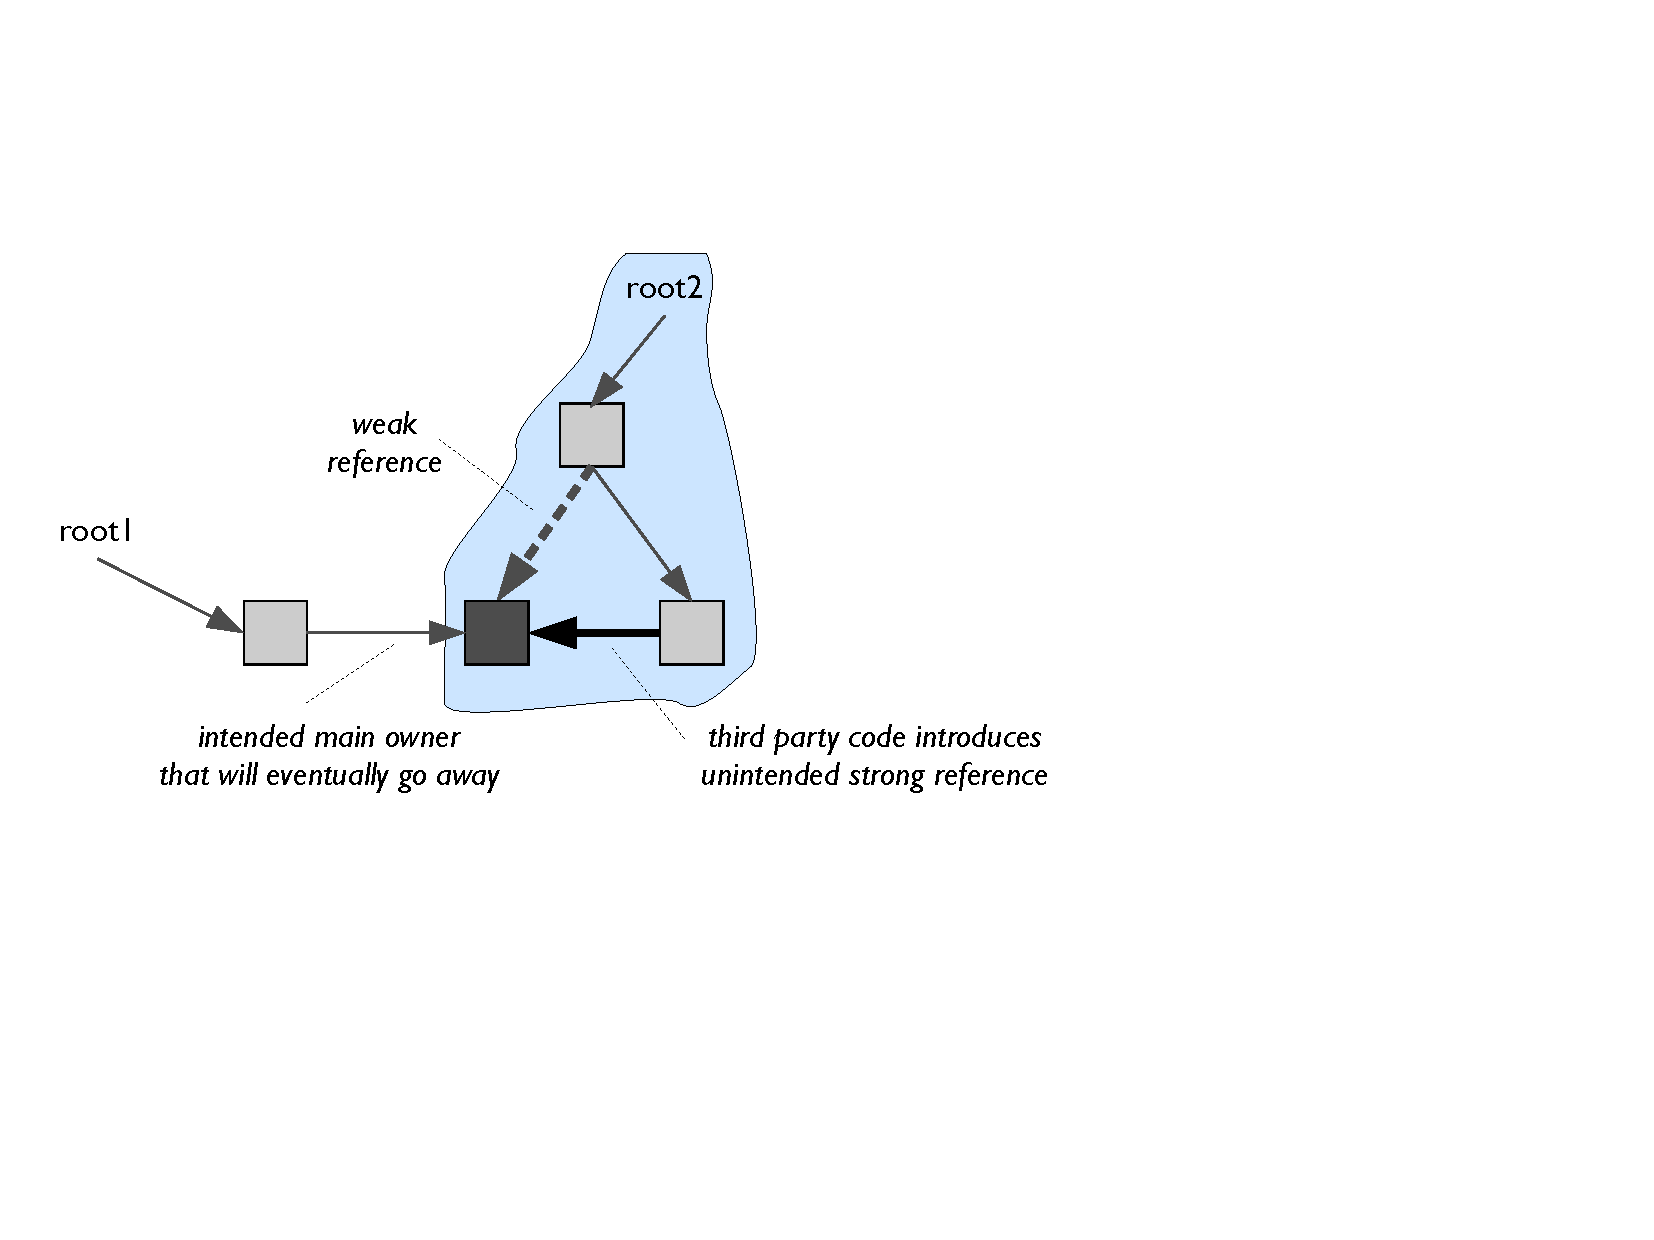
\includegraphics[width=0.6\textwidth]{part4/Figures/lifetime/strongweakdiamonds}
	\caption{Despite your best efforts to use weak references correctly, if you
	introduce a second strong reference in a way that forms a
	\emph{diamond} shape (the shaded region), it will likely never be reclaimed.}
	% [NMM] not sure if we need to give it a name, but, for now
	\label{fig:strongweakdiamonds}
\end{figure}

As is shown in the figure, this problematic reference structure has a diamond
shape. The top of the diamond is the \code{Entry} object of the map, from which
emanate two paths to the key, the weak reference from the \code{Entry} to the
key, and the strong reference path that flows through the value. In
\autoref{fig:strongweakdiamonds}, the darkly shaded object has a good chance of
never being reclaimed. 

In the following code, if \code{loopback} is true, then the \code{Finalized}
message will never appear.
\begin{shortlisting}
static public Object setupCycle(boolean loopback) {
   class Cycle {
       Object loopback;
   }
   class Entry {
       Object key;
       Cycle value;
   }
   Object key = new Object() {
           protected void finalize() {
               System.out.println("Finalized");
           }
       };
   Entry e = new Entry();
   e.key = new WeakReference(key);
   e.value = new Cycle();
   if (loopback) e.value.loopback = key;
   return e;
}
\end{shortlisting}

\paragraph{Finalization and Phantom References}
\index{Finalization of objects}
\index{Phantom References}

Java provides two other closely related cleanup hooks, in the form of
finalization and phantom references. These hooks are called just after the
garbage collector has discovered that the object is collectible, but before its
memory is reclaimed. If you implement a \code{finalize()} method in a class, then
every instance of that class will go through a finalization process. After being
discovered to be garbage, these instances will be enqueued on a special queue,
usually termed the \emph{finalizer queue}. Most \jres spawn a single thread,
termed the finalizer thread, that periodically scans the finalizer queue,
invoking the \code{finalize} method on the enqueued objects.

Phantom references offer a somewhat more refined version of this pre-reclamation
hook. First, with phantom references, you can associate a cleanup hook on a
per-object basis, rather than, as is the case with finalization, on a per-class
basis. Second, phantom references give you the option of having more than one
cleanup queue and thread, in contrast to finalization where there is a single
finalizer queue and (usually) a single finalizer thread.

You can use the hooks offered by finalization or phantom references to free up
resources that are implicitly associated with an object. Any Java objects
uniquely owned by this object will be reclaimed in the normal course of garbage
collection. It is those resources that are \emph{implicitly} tied to a Java
object, such as file descriptors, socket connections, and database resources such
as compiled queries, that require special attention.

You must be very careful in relying on finalization or phantom references. The
Java language specification provides no assurances of how often, or even whether,
finalization will be run on an object. In the normal course of program execution,
eventually the finalizer will run. This is because the finalizer queue consumes
Java heap, and hence the finalizer thread will always do whatever finalization is
possible before the \jre gives up due to heap exhaustion. However, if your Java
objects serve as proxies for some native, or remote, storage, and the space
consumed by the Java proxies is small compared to the external state, then you
may have problems. The \jre knows nothing about this external state, and so will
not schedule the finalizer thread if an external resource is exhausted.

Furthermore, the specification is very lax about whether finalizers will be run
before program termination. You can ask the \jre to attempt to finalize objects
before the program terminates, by calling
\code{System.runFinalizersOnExit(true)}, a deprecated part of the API. However,
most \jres these days run only a partial finalization, if you ask. It is hard for
the \jre to do the right thing in a deadlock free manner. Should it only schedule
the finalizer thread, which would run any pending finalization? This would be
safe, and is what the \jre will do if you ask. But this misses all the
currently-live objects that would have have been finalized, had the program
reached a point where they were reclaimable. The \jre can't unwind, on exit, all
the Java references thta keep those objects alive. Also, there is no analogous
request to have the \jre run a garbage collection on exit. Hence, even for those
objects which are actually ready to be finalized, the \jre won't do so on exit.
It is for these reasons that the API has been deprecated.

Given these downsides, it is best for you to implement a more robust lifetime
management strategy. If you can establish a correlated lifetime pattern, such as
that the external storage should be reclaimed when an event occurs, or when a
method returns, then you should do so.

\paragraph{\TLS}
\tlsindex % \index{\TLS} doesn't seem to work

The last advanced memory management feature offered by Java is the ability to
associate memory with a thread. \Tls provides a way to avoid
synchronization costs, often at the expense of some degree of wasted memory. To
avoid synchronization, you often need to replicate some data structures. This
feature is, of course, only helpful if your program runs with multiple threads.

Consider an example of using the \class{SecureRandom} class. Instances of this
class provide a stream of pseudo-random numbers, in a way that is
cryptographically strong. If you have a singleton instance of this class, you may
experience scalability problems due to lock contention; the contention is hidden
within the \class{SecureRandom} implementation. You can use \tls
to avoid this contention, at the (in this case, small) expense of having one
instance per worker thread:
\begin{shortlisting}
class MyRandomNumberGenerator {
   static ThreadLocal<SecureRandom> rng = new ThreadLocal<SecureRandom>() {
      protected SecureRandom initialValue() {
         SecureRandom random = new SecureRandom();
         random.setSeed(/*some good seed*/);
         return random;
      }
   }
   
   public int next() {
      return rng.get().next(32); // need 32 bits of data
   }
}
\end{shortlisting} 
Java 7 adds a \class{ThreadLocalRandom} implementation to the standard library.

Data stored in \tls will live as long as the thread. If you need
the memory to be reclaimed before the thread terminates, you must explicitly set
the storage to \code{null} via a call to \code{rng.set(null)}. If you are using
the \class{java.util.concurrent} thread pool framework, then you can use its
hooks that are called after a task, or after a thread, terminates. You can do so
by extending the \class{ThreadPoolExecutor} and overriding the
\code{afterExecute} and \code{terminated} methods, respectively.

\Tls, like the \class{WeakHashMap}, is an example of the \jre hiding some of the
complexity of managing weak references. Under the covers, the \tls implementation
uses weak references so that, if a \class{ThreadLocal} object is reclaimed, then
the storage associated with it, for all threads, will be reclaimed, too. In some
implementations, this will not happen immediately, because these implementations
do not use reference queues. They use an alternative approach that at least
keeps the amount of memory spent on stale \tls bounded.
